\documentclass[11pt,a4paper]{article}

% French
\usepackage[utf8x]{inputenc}
\usepackage[frenchb]{babel}
\usepackage[T1]{fontenc}
\usepackage{lmodern}
\usepackage{ifthen}

% Color
% cfr http://en.wikibooks.org/wiki/LaTeX/Colors
\usepackage{color}
\usepackage[usenames,dvipsnames,svgnames,table]{xcolor}
\definecolor{dkgreen}{rgb}{0.25,0.7,0.35}
\definecolor{dkred}{rgb}{0.7,0,0}

% Floats and referencing
\newcommand{\sectionref}[1]{section~\ref{sec:#1}}
\newcommand{\annexeref}[1]{annexe~\ref{ann:#1}}
\newcommand{\figuref}[1]{figure~\ref{fig:#1}}
\newcommand{\tabref}[1]{table~\ref{tab:#1}}
\usepackage{xparse}
\NewDocumentEnvironment{myfig}{mm}
{\begin{figure}[!ht]\centering}
{\caption{#2}\label{fig:#1}\end{figure}}

% Listing
\usepackage{listings}
\lstset{
  numbers=left,
  numberstyle=\tiny\color{gray},
  basicstyle=\rm\small\ttfamily,
  keywordstyle=\bfseries\color{dkred},
  frame=single,
  commentstyle=\color{gray}=small,
  stringstyle=\color{dkgreen},
  %backgroundcolor=\color{gray!10},
  %tabsize=2,
  rulecolor=\color{black!30},
  %title=\lstname,
  breaklines=true,
  framextopmargin=2pt,
  framexbottommargin=2pt,
  extendedchars=true,
  inputencoding=utf8x
}

\newcommand{\matlab}{\textsc{Matlab}}
\newcommand{\octave}{\textsc{GNU/Octave}}
\newcommand{\qtoctave}{\textsc{QtOctave}}
\newcommand{\oz}{\textsc{Oz}}
\newcommand{\java}{\textsc{Java}}
\newcommand{\clang}{\textsc{C}}
\newcommand{\keyword}{mot clef}

% Math symbols
\usepackage{amsmath}
\usepackage{amssymb}
\usepackage{amsthm}
\DeclareMathOperator*{\argmin}{arg\,min}
\DeclareMathOperator*{\argmax}{arg\,max}

% Sets
\newcommand{\Z}{\mathbb{Z}}
\newcommand{\R}{\mathbb{R}}
\newcommand{\Rn}{\R^n}
\newcommand{\Rnn}{\R^{n \times n}}
\newcommand{\C}{\mathbb{C}}
\newcommand{\K}{\mathbb{K}}
\newcommand{\Kn}{\K^n}
\newcommand{\Knn}{\K^{n \times n}}

% Chemistry
\newcommand{\std}{\ensuremath{^{\circ}}}
\newcommand\ph{\ensuremath{\mathrm{pH}}}

% Theorem and definitions
\theoremstyle{definition}
\newtheorem{mydef}{Définition}
\newtheorem{mynota}[mydef]{Notation}
\newtheorem{myprop}[mydef]{Propriétés}
\newtheorem{myrem}[mydef]{Remarque}
\newtheorem{myform}[mydef]{Formules}
\newtheorem{mycorr}[mydef]{Corrolaire}
\newtheorem{mytheo}[mydef]{Théorème}
\newtheorem{mylem}[mydef]{Lemme}
\newtheorem{myexem}[mydef]{Exemple}
\newtheorem{myineg}[mydef]{Inégalité}

% Unit vectors
\usepackage{esint}
\usepackage{esvect}
\newcommand{\kmath}{k}
\newcommand{\xunit}{\hat{\imath}}
\newcommand{\yunit}{\hat{\jmath}}
\newcommand{\zunit}{\hat{\kmath}}

% rot & div & grad & lap
\DeclareMathOperator{\newdiv}{div}
\newcommand{\divn}[1]{\nabla \cdot #1}
\newcommand{\rotn}[1]{\nabla \times #1}
\newcommand{\grad}[1]{\nabla #1}
\newcommand{\gradn}[1]{\nabla #1}
\newcommand{\lap}[1]{\nabla^2 #1}


% Elec
\newcommand{\B}{\vec B}
\newcommand{\E}{\vec E}
\newcommand{\EMF}{\mathcal{E}}
\newcommand{\perm}{\varepsilon} % permittivity

\newcommand{\bigoh}{\mathcal{O}}
\newcommand\eqdef{\triangleq}

\DeclareMathOperator{\newdiff}{d} % use \dif instead
\newcommand{\dif}{\newdiff\!}
\newcommand{\fpart}[2]{\frac{\partial #1}{\partial #2}}
\newcommand{\ffpart}[2]{\frac{\partial^2 #1}{\partial #2^2}}
\newcommand{\fdpart}[3]{\frac{\partial^2 #1}{\partial #2\partial #3}}
\newcommand{\fdif}[2]{\frac{\dif #1}{\dif #2}}
\newcommand{\ffdif}[2]{\frac{\dif^2 #1}{\dif #2^2}}
\newcommand{\constant}{\ensuremath{\mathrm{cst}}}

% Numbers and units
\usepackage[squaren, Gray]{SIunits}
\usepackage{sistyle}
\usepackage[autolanguage]{numprint}
%\usepackage{numprint}
\newcommand\si[2]{\numprint[#2]{#1}}
\newcommand\np[1]{\numprint{#1}}

\newcommand\strong[1]{\textbf{#1}}
\newcommand{\annexe}{\part{Annexes}\appendix}

% Bibliography
\newcommand{\biblio}{\bibliographystyle{plain}\bibliography{biblio}}

\usepackage{fullpage}
% le `[e ]' rend le premier argument (#1) optionnel
% avec comme valeur par défaut `e `
\newcommand{\hypertitle}[7][e ]{
\usepackage{hyperref}
{\renewcommand{\and}{\unskip, }
\hypersetup{pdfauthor={#6},
            pdftitle={Synth\`ese d#1#2 Q#3 - L#4#5},
            pdfsubject={#2}}
}

\title{Synth\`ese d#1#2 Q#3 - L#4#5}
\author{#6}

\begin{document}

\ifthenelse{\isundefined{\skiptitlepage}}{
\begin{titlepage}
\maketitle

 \paragraph{Informations importantes}
   Ce document est grandement inspiré de l'excellent cours
   donné par #7 à l'EPL (École Polytechnique de Louvain),
   faculté de l'UCL (Université Catholique de Louvain).
   Il est écrit par les auteurs susnommés avec l'aide de tous
   les autres étudiants, la vôtre est donc la bienvenue.
   Il y a toujours moyen de l'améliorer, surtout si le cours
   change car la synthèse doit alors être modifiée en conséquence.
   On peut retrouver le code source à l'adresse suivante
   \begin{center}
     \url{https://github.com/Gp2mv3/Syntheses}.
   \end{center}
   On y trouve aussi le contenu du \texttt{README} qui contient de plus
   amples informations, vous êtes invité à le lire.

   Il y est indiqué que les questions, signalements d'erreurs,
   suggestions d'améliorations ou quelque discussion que ce soit
   relative au projet
   sont à spécifier de préférence à l'adresse suivante
   \begin{center}
     \url{https://github.com/Gp2mv3/Syntheses/issues}.
   \end{center}
   Ça permet à tout le monde de les voir, les commenter et agir
   en conséquence.
   Vous êtes d'ailleurs invité à participer aux discussions.

   Vous trouverez aussi des informations dans le wiki
   \begin{center}
     \url{https://github.com/Gp2mv3/Syntheses/wiki}.
   \end{center}
   comme le statut des synthèses pour chaque cours
   \begin{center}
     \url{https://github.com/Gp2mv3/Syntheses/wiki/Status}.
   \end{center}
   vous pouvez d'ailleurs remarquer qu'il en manque encore beaucoup,
   votre aide est la bienvenue.

   Pour contribuer au bug tracker et au wiki, il vous suffira de
   créer un compte sur Github.
   Pour interagir avec le code des synthèses,
   il vous faudra installer \LaTeX.
   Pour interagir directement avec le code sur Github,
   vous devez utiliser \texttt{git}.
   Si cela pose problème,
   nous sommes évidemment ouverts à des contributeurs envoyant leurs
   changements par mail ou n'importe quel autre moyen.
\end{titlepage}
}{}

\ifthenelse{\isundefined{\skiptableofcontents}}{
\tableofcontents
}{}
}


\usepackage{pgfplots}
\usepackage{caption}
\usepackage{subcaption}
\usepackage{xspace}

\hypertitle{fr}{Physique}{3}{FSAB}{1203}
{Ga\"{e}tan Cassiers\and Nicolas Cognaux\and Benoît Legat\and Antoine Legat\and Antoine Paris}
{Jérôme Louveaux, Claude Oestges et Jean-Christophe Charlier}

\part{Ondes}
%   _     _     _     _     _     _     _...
%  / \   / \   / \   / \   / \   / \   / ...
% /   \_/   \_/   \_/   \_/   \_/   \_/  ...
\section{Courant de déplacement}
La loi d'ampère
\[ \oint \vec{B} \cdot \dif \vec{l} = \mu_0 \int \vec{J} \cdot \dif \vec{A} \]
est incohérente dans certains cas (exemple du condensateur).

Il faut rajouter un terme appelé \emph{courant de déplacement}
pour qu'elle soit correcte dans tous les cas.
Ce courant est déterminé par
\[ \vec{J}_\mathrm{D} = \perm_0\fpart{\vec{E}}{t} \]
et l'équation d'Ampère correcte est alors
\[ \oint \vec{B} \cdot \dif \vec{l} =
\mu_0 \int \vec{J} \cdot \dif \vec{A} +
\mu_0\perm_0 \int\fpart{\vec{E}}{t} \cdot \dif \vec{A}. \]

Le courant de déplacement n'est pas vraiment un courant (déplacement de charges),
mais il est équivalent : il permet de représenter le \og courant\fg qui
circule dans un condensateur (et donc de vérifier la loi des n\oe{}uds
(loi de Kirchoff) dans tous les cas).

\section{Équations de Maxwell}
On peut résumer toutes les lois qui gouvernent l'électromagnétisme
par 4 lois que les théorèmes intégraux nous permettent de réécrire
de 2 manières différentes
\begin{align*}
  &\text{Gauss} & \oint \E \cdot \dif \vec{A} & = \frac{Q}{\perm}
  & \divn{\E} & = \frac{\rho}{\perm}\\
  &\text{No monopôle magn.} & \oint \B \cdot \dif \vec{A} & = 0
  & \divn{\B} & = 0\\
  &\text{Lenz-Faraday} & \oint \E \cdot \dif \vec{l} & = -\fpart{}{t} \int \B \cdot \dif \vec{A}~~~\text{\footnotemark}
  & \rotn{\E} & = -\fpart{\B}{t}\\
  &\text{Maxwell-Ampère} & \oint \B \cdot \dif \vec{l} & = \mu \int \vec{J} \cdot \dif \vec{A}
  + \mu\perm\fpart{}{t} \int \E \dif \vec{A}
  & \rotn{\B} & = \mu\vec{J} + \mu\perm\fpart{\E}{t}
\end{align*}
\footnotetext{Les physiciens qui aiment la symétrie cherchent un terme supplémentaire ici.}

avec
\begin{align*}
  \vec{E} & = -\gradn{V}\\
  Q & = \int \rho \dif V.
\end{align*}

\section{Ondes}
\subsection{Équation d'onde et équations de propagation}
Une onde est un phénomène de propagation d'une quantité \(\vec{u}\)
 qui vérifie l'\emph{équation d'onde}
\begin{equation*}\begin{split}
\frac{\partial^2 u}{\partial t^2} &= v^2 \lap u \\
 &= v^2 \left(
 \frac{\partial^2 u}{\partial x^2} +
 \frac{\partial^2 u}{\partial y^2} +
 \frac{\partial^2 u}{\partial z^2}\right)
\end{split}\end{equation*}

Lorsque deux grandeurs sont liées par les \emph{équations de propagation}
\begin{equation}\begin{split}\label{eq:propagation}
    \nabla A & = -a \frac{\partial B}{\partial t} \\
    \frac{\partial A}{\partial t} & = -b \nabla B
\end{split}\end{equation}
elles obéissent toutes les deux à la même équation d'onde
\begin{align*}
\dfrac{\partial^2 A}{\partial t^2} &= v^2 \lap A
& \dfrac{\partial^2 B}{\partial t^2} &= v^2 \lap B
\end{align*}
avec \[v = \sqrt{\frac{b}{a}}.\]

Il existe deux types d'ondes,
\begin{itemize}
  \item les ondes transverses où $\vec{u} \perp \vec{v}$ (par exemple une corde);
  \item les ondes longitudinales où $\vec{u} \parallel \vec{v}$ (ex: le son).
\end{itemize}

\subsection[Cas particuliers]{Solution de l'équation d'onde dans des cas particuliers}
\subsubsection{Onde 1D}
On peut se demander s'il existe une fonction à une variable $C(w)$ vérifiant
l'équation d'onde à une dimension, c'est-à-dire $C(w) = u(x,t)$,
et si oui quelle est l'expression de $w(x,t)$.
La réponse est oui, si on prend $w(x,t) = x \pm\footnote{En fait, le signe importe peu, vu que $v$ peut être positif ou négatif (car il y a seulement $v^2$ dans l'équation d'onde).} vt$\footnote{ou tout multiple de $w$.},
on vérifie\footnote{à l'aide de la \textit{Chain rule}.}
\[ \dfrac{\partial^2 C(w)}{\partial t^2} =
v^2 \dfrac{\partial^2 C(w)}{\partial x^2}\]

Cela correspond bien à l'intuition. En effet, c'est comme si on avait une fonction $C(x)$
(p. ex. une sinusoïde ou un gaussienne) qui se déplaçait dans le temps à une vitesse $v$.

Si $v$ est positif, l'équation $w(x,t) = x - vt$ correspond à une onde se déplaçant vers
les $x$ croissants, tandis que $w(x,t) = x + vt$ correspond à une onde qui se déplace vers
les $x$ décroissants.

L'équation d'onde en 1D est donc
\begin{equation}u(x, t) = f(x - vt)\label{eq:onde1D}\end{equation}
Pour les ondes périodiques, on écrit souvent cette équation $u(x, t) = f(kx-\omega t)$
(voir \ref{sec:onde_sin}).

En l'absence de constante d'intégration\footnote{
    Le champ magnétique de la Terre dans le cas d'une onde EM,
    la hauteur de la corde au repos dans le cas d'une corde vibrante ...},
le rapport de $A$ sur $B$ (variables des équations de propagation \eqref{eq:propagation})
vaut une constante particulière dénotée $Z$ et appelée l'\emph{impédance caractéristique}
\footnote{Par exemple, l'impédance caractéristique d'un milieu pour une onde acoustique
représente la résistance du milieu au passage de cette onde.}
\[\dfrac{A(x,t)}{B(x,t)} = Z = \sqrt{ab}\]

\subsubsection{Onde 3D : cas symétriques}\label{sec:cas_symetriques}
Dans certains cas symétriques, on se ramène au cas 1D:
\begin{itemize}
\item Onde plane :
\begin{equation}f(\vec{k}\cdot\vec{x}\pm\omega t)\label{eq:expr_onde_plane}\end{equation} avec
$\vec{x}$ le vecteur position du point et $\vec{k}$ le vecteur d'onde, c'est
à dire un vecteur dont la norme est le nombre d'onde $k$ et dont la direction
est perpendiculaire au front d'onde (et donc parallèle à la direction
de propagation de l'onde) ;
\item Onde cylindrique : \(f(k\rho\pm\omega t)\) avec \(\rho = \sqrt{x^2+y^2}\) ;
\item Onde sphérique : \(f(kr\pm\omega t)\) avec \(r = \sqrt{x^2+y^2+z^2}\).
\end{itemize}

\subsubsection{Onde sinusoïdale}\label{sec:onde_sin}
Une onde sinusoïdale 1D a l'équation suivante
\begin{equation}\label{eq:onde_sin}
A(x, t) = A_0 \sin(kx - \omega t + \phi)
\footnote{Cette expression est donnée dans le cas 1D
(c'est un cas particulier de l'équation \eqref{eq:onde1D}) mais on peut
bien sûr généraliser aux cas 3D symétriques (voir section \ref{sec:cas_symetriques}).}
\end{equation}
et les caractéristiques suivantes
\begin{itemize}
  \item $A_0$, son amplitude, c'est à dire son intensité maximale;
  \item $x$, la position du point;
  \item $\omega$, sa vitesse angulaire;
  \item $f$, sa fréquence d'oscillation;
  \item $T$, sa période d'oscillation;
  \item $k$, le nombre d'onde;
  \item $\lambda$, la longueur d'onde;
  \item $v$, sa vitesse de propagation;
  \item $\phi$, une phase.
\end{itemize}
Elles sont liées entre elles par les relations suivantes
\begin{align*}
  T & = \frac{1}{f}\\
  \omega & = 2\pi f\\
  v & = \lambda f\\
  k & = \frac{2\pi}{\lambda}
\end{align*}

\subsection{Ondes électromagnétiques}
\subsubsection{Propriétés}
Les ondes électromagnétiques sont des ondes transverses
de $\vec{E}$ et $\vec{B}$.

Leur vitesse de propagation est $c$ (vitesse de la lumière).

On a les relations supplémentaires\footnote{Ces relations peuvent
être déduites pour un cas particulier d'onde
électromagnétique relativement simple (les ondes électromagnétiques
planes) en vérifiant la validité des lois d'Ampère et de Faraday.
Elles sont cependant valables pour \emph{toutes} les ondes
électromagnétiques.}
\begin{align*}
  \vec{E} & \perp \vec{B}\\
  c & = \frac{1}{\sqrt{\perm\mu}}\\
  \frac{E}{B} & = c.
\end{align*}

La direction de propagation d'une onde électromagnétique est
donnée par la direction de $\vec{E} \times \vec{B}$.
Le spectre des ondes électromagnétiques est présenté à
la figure \ref{fig:em-spectrum}.

\begin{figure}[ht]
	\centering
	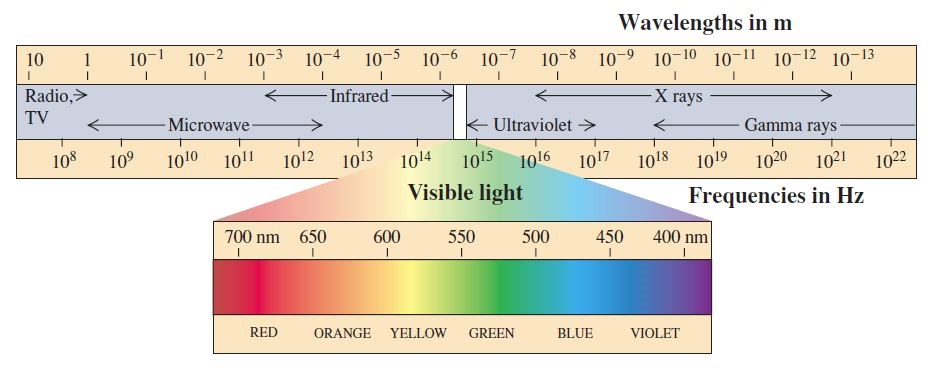
\includegraphics[scale=0.8]{em-spectrum.jpg}
	\caption{Spectre des ondes électromagnétiques.}
	\label{fig:em-spectrum}
\end{figure}

\subsubsection{Équations de propagation et équation d'onde}
En émettant les hypothèses que $\vec{E}$ est suivant $\hat{y}$ et $\vec{H}$ suivant $\hat{z}$ et à l'aide des équations de Maxwell
\footnote{Sous l'hypothèse que $\vec{J}=0$. Dans le vide ce sera toujours le cas.}, on trouve que $\vec{E}$ et $\vec{H}$ ne dépendent
que de leur abscisse $x$. Les champs électrique et magnétique sont donc constants le long d'un plan perpendiculaire 
à l'axe des abscisses. On obtient également les équations de propagation d'une onde électromagnétique
\begin{align*}
\fpart{E_y}{x} &= -\mu \fpart{H_z}{t} & \fpart{H_z}{x} &= -\perm \fpart{E_y}{t}.
\end{align*}

En appliquant $\fpart{}{t}$ et $\fpart{}{x}$ à ces relations, on obtient l'équation d'onde de $H_z$ et $E_y$ respectivement
\begin{align*}
\dfrac{\partial^2 H_z}{\partial t^2} &=
c^2 \dfrac{\partial^2 H_z}{\partial x^2}
& \dfrac{\partial^2 E_y}{\partial t^2} &=
c^2 \dfrac{\partial^2 E_y}{\partial x^2}.
\end{align*}

Cela permet de calculer l'impédance caractéristique,
\[
Z = \sqrt{\dfrac{\mu}{\perm}} \overset{\text{si dans le vide}}{=} \sqrt{\dfrac{\mu_0}{\perm_0}} = \unit{120\pi}{\ohm},
\]
et dépend donc du milieu.

On a montré qu'un champ électromagnétique peut se propager dans le vide
(ou dans la matière) sous la forme d'une onde. Cette onde peut avoir différentes
caractéristiques selon l'émetteur (antenne...).
Un cas fréquent est l'onde plane sinusoïdale (\eqref{eq:expr_onde_plane} et
\eqref{eq:onde_sin}).

\subsubsection{Densité d'énergie d'une onde électromagnétique}
En se rappelant de la densité d'énergie d'un champ électrique et
d'un champ magnétique, on peut écrire

$$u = u_E + u_M = \frac{\perm E^2}{2} + \frac{B^2}{2\mu}.$$

Or on sait que $B = \frac{E}{c} = E\sqrt{\perm\mu}$, on a donc

$$u = \unit{\perm E^2}{\joule\per\meter\cubed}$$

\subsubsection{Intensité d'une onde électromagnétique}
L'intensité d'une onde électromagnétique, c'est à
dire la densité de puissance véhiculée par l'onde, est calculée
en multipliant la densité d'énergie par la vitesse de propagation

$$I = cu = \unit{c\perm E^2}{\watt\per\meter\squared}$$

De manière plus générale, on défini le \emph{vecteur de Poynting}

\[\vec{S} = \vec{E} \times \vec{H} = \frac{1}{\mu} \vec{E} \times \vec{B}\]

dont la direction est parallèle à la direction de propagation de l'onde électromagnétique
et la norme en est l'intensité.

\paragraph{Intensité et types d'ondes}
Selon le front d'onde\footnote{Le front d'onde est la surface d'égale phase d'une onde,
c'est à dire que ses points ont mis le même temps de parcours depuis la source.},
l'intensité varie différemment en fonction de la distance à la source.
\begin{itemize}
	\item Pour une onde plane : $E(r,t) = E_0f(r-vt)$, l'intensité est constante ;	
	\item Pour une onde cylindrique : $E(r,t) = \frac{E_0}{\sqrt{r}}f(r-vt)$, l'
	intensité varie en $\frac{1}{r}$ ;
	\item Pour une onde sphérique : $E(r,t) = \frac{E_0}{r}f(r-vt)$, l'intensité
	varie en $\frac{1}{r^2}$.
\end{itemize}
On visualise facilement pourquoi grâce aux figures \ref{fig:onde-cyl} et
\ref{fig:onde-sph}.

% TODO : find better images...
\begin{figure}[ht]
	\centering
	\begin{subfigure}[b]{0.45\textwidth}
		\centering
		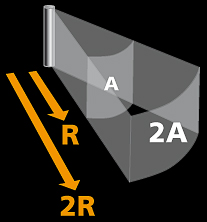
\includegraphics[scale=0.6]{cylindrical-wavefront.jpg}
		\caption{Onde cylindrique (source linéique).}
		\label{fig:onde-cyl}
	\end{subfigure}
	\begin{subfigure}[b]{0.45\textwidth}
		\centering
		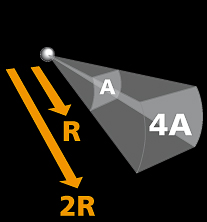
\includegraphics[scale=0.6]{spherical-wavefront.jpg}
		\caption{Onde sphérique (source ponctuelle).}
		\label{fig:onde-sph}
	\end{subfigure}
	\caption{Fronts d'ondes.}
\end{figure}

\paragraph{Onde sinusoïdale} L'intensité moyenne d'une onde EM sinusoïdale vaut
\[I_m = \frac{\epsilon c E^2_{max}}{2}\]

\subsection{Ondes mécaniques}
Il est important, pour commencer, d'insister sur le fait
que les ondes transportent de l'énergie et de la quantité de mouvement,
et non de la matière d'un point à un autre.

\subsubsection{Corde}
On peut appliquer une onde transverse dans une corde.
Si la corde est tendue avec une force $F$ et que
sa masse linéique $[\kilogram\per\meter]$ est $m_L$,
la vitesse de propagation d'une telle onde est
\[ v = \sqrt{\frac{F}{m_L}}. \]

\subsubsection{Son}
Le son est une onde longitudinale de compression de l'air.
La vitesse de propagation du son dans l'air à \si{298}{K} et \si{1}{atm}
$v = \si{344}{\meter\per\second}$.

La vitesse du son varie avec la température, suivant la loi des gaz parfaits.
Nous avons donc la relation $v = \sqrt{\frac{B}{\rho_0}} \simeq 20.1\sqrt{T}$

Pour mesurer l'intensité d'une onde, on utilise une échelle logarithmique
\[ I[\deci\bel] = 10 \log_{10}\frac{I[\watt\per\meter\squared]}{I_0} \]
où $I_0 = \si{1e-12}{\watt\per\meter\squared}$.

\paragraph{Décibel}

Permet d'exprimer un rapport de puissances ou d'intensités
(pas uniquement du son !)
\[\text{rapport [dB] } = 10 \log_{10}\frac{I_1}{I_2}\]
Pour un rapport d'amplitudes, tensions\dots \(A\) tel que \(I \propto A^2\) :
\[\text{rapport [dB] } = \strong{20} \log_{10}\frac{A_1}{A_2}\]

\subsection{Effet Doppler}
Soit une source se déplaçant à une vitesse $v_s$ et émettant
une onde de vitesse $v$ et de fréquence $f_s$.
Soit un observateur se déplaçant à une vitesse $v_o$ et
observant cette onde à une fréquence $f_o$.

On suppose que les trois vitesses sont parallèles.

\subsubsection{Pour une onde non-électromagnétique}
Si on a $v \ll c$, on peut dire que
\[ f_o = \frac{v \pm v_o}{v \pm v_s} f_s. \]

Il faut utiliser le bon sens pour savoir si c'est un plus ou un moins.
Par exemple, si la source se rapproche de l'observateur, et que
l'observateur se rapproche de la source, les deux vitesses
tendent à augmenter la fréquence perçue par l'observateur donc
\[ f_o = \frac{v + v_o}{v - v_s} f_s. \]

\begin{myrem}
	Pour une onde non-électromagnétique, on ne peut pas simplement
	utiliser la vitesse relative de l'observateur et de la source
	(voir exercice 16.48 du Young And Freedman).
\end{myrem}

\subsubsection{Pour une onde électromagnétique}
Lorsqu'on applique l'effet Doppler aux ondes électromagnétiques,
on ne s'intéresse plus à la vitesse de l'observateur et de la source séparément
mais à leur vitesse relative $u$ avec $u$ \emph{positif} s'ils se rapprochent
et \emph{négatif} s'ils s'éloignent.

La relativité nous permet de montrer que
\[ f_o = \sqrt{\frac{c + u}{c - u}}f_s. \]
Si $u \ll c$, on a
\[ \frac{f_o - f_s}{f_s} \approx \frac{u}{c}. \]

\paragraph{Attention} Parfois, il faut appliquer l'effet Doppler deux fois
comme pour un radar où l'objet est d'abord observateur et le radar la source
avant que les rôles ne s'inversent.
On a alors
\[ f_o = \frac{c + u}{c - u}f_s \]
et si $u \ll c$
\[ \frac{f_o - f_s}{f_s} \approx \frac{2u}{c}. \]

\section{Polarisation, réflexion et réfraction}

\subsection{Polarisation}
Le type de polarisation indique la forme du lieu parcouru
par l'extrémité du vecteur (souvent champ électrique) associé à un
point de l'espace.

Supposons que l'onde se déplace selon $\vec{z}$,
une polarisation générale serait
\[ \vec{E}(\vec{r}, t) = A_x \sin(\vec{k}\cdot\vec{r} - \omega t + \phi_1)
  \xunit
+ A_y \sin(\vec{k} \cdot \vec{r} - \omega t + \phi_2) \yunit \]
C'est ce qu'on appelle on polarisation elliptique.
Il y a deux cas dégénérés:
\begin{itemize}
  \item Si $\phi_2-\phi_1 = \pm \frac{\pi}{2}$
    et $A_x = A_y$, c'est une polarisation circulaire;
  \item Si $\phi_2-\phi_1 = 0$ ou $\pm\pi$ ou si $A_x = 0$ ou $A_y = 0$,
    c'est une polarisation linéaire.
\end{itemize}

\subsection{Réflexion et réfraction}
Lorsqu'une onde passe d'un milieu à un autre,
elle se réfléchit en une onde \emph{réfléchie} et se réfracte en une onde
\emph{transmise} à la surface de séparation des deux milieux.

\paragraph{Attention}
Une onde électromagnétique ne passe pas à travers une membrane métallique,
elle y est réfléchie.

\subsubsection{Réflexion}

Lors de la réflexion, les paramètres $\omega$, $f$, $v$ et $\lambda$
sont identiques à ceux de l'onde incidente.
L'angle de réflexion est égal à l'angle d'incidence.

L'onde réfléchie n'est pas toujours en phase avec l'onde incidente.
Elle est soit en phase, soit déphasée de $\pi$.

En fait, si le coefficient donné par l'équation de Fresnel est positif,
elle est en phase, sinon elle est déphasée (c.-à-d. en opposition de phase).
C'est à dire que:
\begin{itemize}
  \item Si $n_1 < n_2$, la réflexion de la partie de l'onde
    qui est perpendiculaire au plan
    d'incidence est déphasée de $\pi$ avec l'onde incidente
    et celle de la partie parallèle est déphasée de $\pi$
    pour $\theta < \theta_b$;
  \item Si $n_1 > n_2$, la réflexion de la partie perpendiculaire est
    en phase et celle de la partie parallèle est déphasée de $\pi$
    pour $\theta_b < \theta$.
\end{itemize}

\subsubsection{Réfraction}
L'onde transmise a la même vitesse angulaire $\omega$
et la même fréquence $f$ que l'onde incidente
mais pas la même vitesse $v$ ni la même longueur d'onde $\lambda$.

Elle est en phase avec l'onde incidente.

\paragraph{Indice de réfraction}
On définit les indices de réfraction comme suit
\[ \frac{n_1}{n_2} \eqdef \frac{v_2}{v_1} = \frac{\lambda_2}{\lambda_1} \]

Dans le cas d'une onde électromagnétique,
$v = c = \frac{1}{\sqrt{\perm\mu}}$.
En définissant $n_\mathrm{vide} = 1$,
on a alors
$n = \sqrt{\perm_r\mu_r}$.

\paragraph{Loi de Snell-Descartes}
L'angle transmis $\theta_2$ par rapport à l'angle d'incidence
$\theta_1$ nous est donné par la loi de \emph{Snell-Descartes}
\begin{equation}
  \label{eq:snell}
  n_1 \sin(\theta_1) = n_2 \sin(\theta_2).
\end{equation}

\subsubsection{Équations de Fresnel}
Pour trouver l'intensité de l'onde réfléchie et transmise, il nous
faut décomposer son intensité en une composante parallèle au plan d'incidence
\footnote{La plan d'incidence est le plan contenant la normale à la surface
et le vecteur d'onde de l'onde incidente.}
$E^\parallel$ et une perpendiculaire $E^\perp$.

Soit $E_{1r}$ l'intensité du champ réfléchi
et $E_{2}$ l'intensité du champ transmis.
On a les formules suivantes
\begin{align*}
  E_{1r}^\parallel & = \frac{n_1\cos\theta_2 - n_2\cos\theta_1}
  {n_1\cos\theta_2 + n_2\cos\theta_1}E_{1}^\parallel
  \stackrel{\eqref{eq:snell}}{=}
  \frac{\tan(\theta_2 - \theta_1)}{\tan(\theta_2 + \theta_1)}E_1^\parallel
  & E_2^\parallel & = \frac{2n_1\cos(\theta_1)}
  {n_1\cos\theta_2 - n_2\cos\theta_1}E_{1}^\parallel\\
  E_{1r}^\perp & = \frac{n_1\cos\theta_1 - n_2\cos\theta_2}
  {n_1\cos\theta_1 + n_2\cos\theta_2}E_{1}^\perp
  \stackrel{\eqref{eq:snell}}{=}
  \frac{\sin(\theta_2 - \theta_1)}{\sin(\theta_2 + \theta_1)}E_1^\perp
  & E_2^\perp & = \frac{2n_1\cos(\theta_1)}
  {n_1\cos\theta_1 - n_2\cos\theta_2}E_{1}^\perp\\
\end{align*}
Les graphes de ces coefficients se trouvent
sur les figures \ref{fig:fresnel-1} et \ref{fig:fresnel-2}.

\begin{figure}[ht]
	\centering
	\begin{subfigure}[b]{0.45\textwidth}
		\centering
		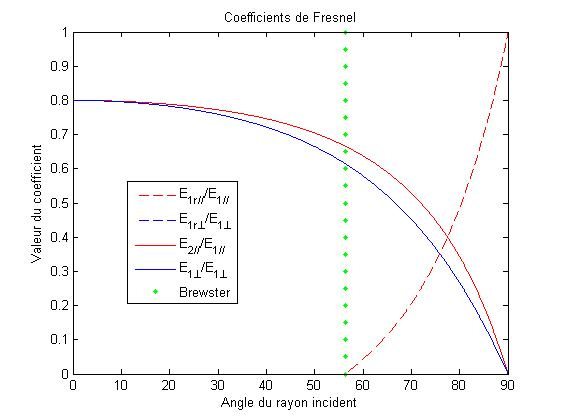
\includegraphics[scale=0.4]{fresnel-1.jpg}
		\caption{Valeurs des coéfficients de Fresnel pour $n_1 = 1.0$ et $n_2 = 1.5$.}
		\label{fig:fresnel-1}
	\end{subfigure}
	\begin{subfigure}[b]{0.45\textwidth}
		\centering
		% fresnel-2.jpg encore à faire proprement
		\includegraphics[scale=0.4]{fresnel-2.jpg}
		\caption{Valeurs des coéfficients de Fresnel pour $n_1 = 1.5$ et $n_2 = 1.0$.}
		\label{fig:fresnel-2}
	\end{subfigure}
	\caption{Graphes des coefficients de Fresnel.}
\end{figure}

\begin{myrem}
	Puisque les composantes perpendiculaires et parallèles
	du champs changent, il est évident que l'angle de polarisation
	par rapport au plan d'incidence changent également (voir
	exercice 8 de l'APE4).
\end{myrem}

\paragraph{Angle de Brewster}
Il existe un angle pour lequel $E_{1r}^\parallel = 0$,
on l'appelle l'angle de Brewster et c'est l'angle $\theta_B$ tel que
\[ \tan\theta_B = \frac{n_2}{n_1}. \]

\paragraph{Angle critique}
Si $n_1 > n_2$, il existe un angle critique $\theta_{1c}$ tel que
$E_{2} = 0$ pour tout $\theta_1 \geq \theta_{1c}$.
C'est l'angle qui respecte
\[ \sin\theta_{1c} = \frac{n_2}{n_1}. \]

On voit bien ici pourquoi, si $n_1 < n_2$, cet angle n'existe pas.

\section{Interférence et diffraction}
Quand une onde traverse une fente ou un objet, elle subit une diffraction.
Si c'est un objet et non une fente, l'effet est le même,
on ne traitera donc que le cas de fentes.
On considère aussi que le point où on mesure l'onde est loin des fentes
par rapport à leur distance entre elles.

\subsection{Approximation de Fraunhofer}
\label{sec:fraunhofer}
Lorsqu'il faut estimer la différence de distance entre différentes
fentes ou antennes situées aux points $P_i$ émettant des ondes
et un point $P$ loin d'elles,
il est nécessaire de faire l'approximation de Fraunhofer qui
consiste à considérer que tous les vecteurs $\vec{P_iP}$
sont parallèles.
La distance supplémentaire d'une fente à l'autre est donc $d\sin\theta$
où $d$ est la distance entre deux fentes et $\theta$ l'angle
formé avec la perpendiculaire aux deux fentes.

\subsection{Interférence}
Si une onde arrive sur deux fentes de largeur négligeable séparées par
une distance $d$,
il y aura interférence constructive si $\exists n \in \mathbb{N}$ tel que
\[ d\sin\theta = n \lambda \]
et interférence destructive si $\exists n \in \mathbb{N}$ tel que
\[ d\sin\theta = \left(n+\frac{1}{2}\right) \lambda \].

Si on considère $N$ fentes de largeur négligeable séparées par une
distance $d$ (voir figure \ref{fig:interference}),
\[ I(P) \propto \frac{A^2}{R^2} \cdot
  \frac{\sin^2\left(\frac{N \pi d \sin\theta}{\lambda}\right)}
{\sin^2\left(\frac{\pi d \sin\theta}{\lambda}\right)} \]
où $R$ est la distance entre $P$ et la fente la plus proche
et $A$ est l'amplitude de l'onde incidente.

Ce qui donne des minimas si
$\exists n \in \mathbb{N}_0$ non divisibles par $N$ tel que
\[ N d \sin \theta = n \lambda \]
et des maxima si $\exists n \in \mathbb{N}$ tel que
\[ d \sin \theta = n \lambda. \]

\begin{figure}[ht]
	\centering
	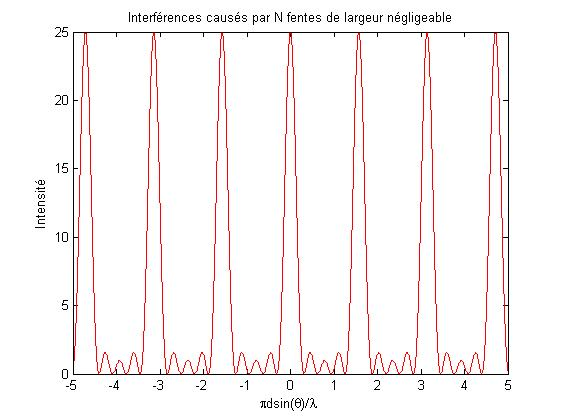
\includegraphics[scale=0.5]{interference.jpg}
	\caption{Intensité de l'interférence d'une ondes par $N$ fentes de largeur négligeable.}
	\label{fig:interference}
\end{figure}

\subsubsection{Interférence sur un film mince}
Soit un film mince d'épaisseur $d$ illuminé par une onde
plane. Il y a ici 3 milieux à considèrer :

\begin{enumerate}
	\item Le milieu 0 (situé au dessus du film) d'indice
	de réfraction $n_0$, dans ce milieu l'onde a une longueur
	d'onde $\lambda_0$ ;
	\item Le milieu 1 (dans le film) d'indice de réfraction
	$n_1$, dans ce milieu l'onde a une longueur d'onde $\lambda_1$ ;
	\item Le milieu 2 (en dessous du film) d'indice de réfraction
	$n_2$, dans ce milieu l'onde a une longueur d'onde $\lambda_2$ ;
\end{enumerate}

Les différents angles d'incidences sont représentés sur la
figure \ref{fig:film-mince}.

%TODO figure à refaire si quelqu'un a le temps...
\begin{figure}[ht!]
	\centering
		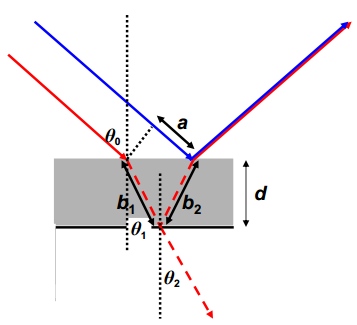
\includegraphics[scale=1.0]{film-mince.png}
		\caption{Un film mince illuminé par une onde plane.}
		\label{fig:film-mince}
\end{figure}

Le déphasage $\Delta \Phi$ entre deux rayons
réfléchis (le rouge et le bleu sur la figure \ref{fig:film-mince})
est donné par

$$\Delta \Phi = \frac{4\pi dn_1}{n_0\lambda_0}\cdot\cos(\theta_1) + \alpha_1$$

où $\alpha_1$ vaut 0 ou $\pi$ selon le déphasage dû à la
réflexion ou à la réfraction aux interfaces (voir signes
des coéfficients des équations de Fresnel).
La couleur associé à $\lambda_0$ sera plus perçue si

$$\Delta \Phi = 2m\pi$$

ou sera moins perçue si

$$\Delta \Phi = (2m+1)\pi.$$

C'est en se basant sur ce principe que l'on peut
fabriquer des couches anti-reflets ou, au contraire,
des couches réflectrices.

\subsubsection{Figure d'interférences}
La superposition d'ondes donne lieu à une \emph{figure
d'interférences}. Sur ces figures d'interférence, on
peut distinguer les lignes nodales et les lignes anti-nodales.
Les lignes nodales (en jaune sur la figure \ref{fig:nodale})
représentent le lieu des interférences destructives tandis que
les lignes anti-nodales (en bleu sur la figure \ref{fig:antinodale})
représentent le lieu des interférences constructives.

% TODO : trouver des figures un peu mieux
\begin{figure}[ht]
	\centering
	\begin{subfigure}[b]{0.45\textwidth}
		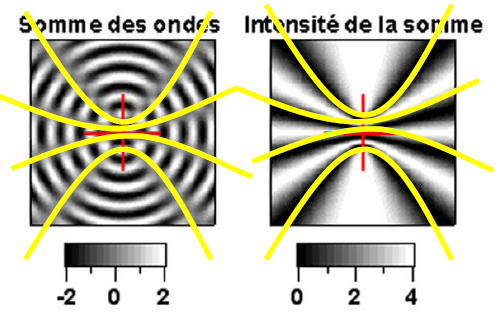
\includegraphics[scale=0.8]{fig_interferences_nodales.png}
		\caption{Lignes nodales.}
		\label{fig:nodale}
	\end{subfigure}
	\begin{subfigure}[b]{0.45\textwidth}
		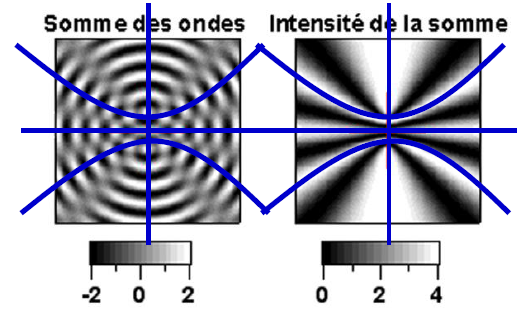
\includegraphics[scale=0.8]{fig_interferences_antinodales.png}
	\caption{Lignes anti-nodales.}
	\label{fig:antinodale}
	\end{subfigure}
	\caption{Figure d'interférence entre deux sources de même fréquence.}
\end{figure}

\subsubsection{Applications}
Les interférences permettent de redistribuer spatialement l'énergie,
et donc de diriger l'énergie vers certaines régions de l'espace.
Les interférences sont donc utilisées, par exemple pour les antennes
GSM.

%TODO : diagramme polaire (vraiment utile?),représentation complexe d'une onde
%(en annexe?),interféromètre de Michelson

\subsection{Diffraction}
Supposons maintenant que l'épaisseur $a$ des fentes n'est plus
négligeable.
\begin{itemize}
  \item Pour une fente rectangulaire (voir figure \ref{fig:diffraction1}),
    \[ I(P) \propto I_0 \times
      \frac{\sin^2\left(\frac{\pi a \sin\theta}{\lambda}\right)}
    {\left(\frac{\pi a \sin\theta}{\lambda}\right)^2}; \]
  \item et pour $N$ fentes (voir figure \ref{fig:diffractionN}),
    \[ I(P) \propto I_0 \times
      \frac{\sin^2\left(\frac{\pi a \sin\theta}{\lambda}\right)}
      {\left(\frac{\pi a \sin\theta}{\lambda}\right)^2} \times
      \frac{\sin^2\left(\frac{N \pi d \sin\theta}{\lambda}\right)}
    {\sin^2\left(\frac{\pi d \sin\theta}{\lambda}\right)}. \]
\end{itemize}
On a des minima si $\exists n \in \mathbb{N}_0$ tel que
\[ a \sin \theta = n\lambda. \]

Si $N \neq 1$, on a aussi les minimas et maximas qu'avait
l'interférence à $N$ fentes.
Sauf bien sûr, les maximas pour lesquels $a\sin\theta = n\lambda$.
Par exemple, si $a = \frac{d}{2}$, tous les maximas d'ordre pairs
seront \emph{éteints}.

\begin{figure}[ht]
	\centering
	\begin{subfigure}[b]{0.45\textwidth}
		\centering
		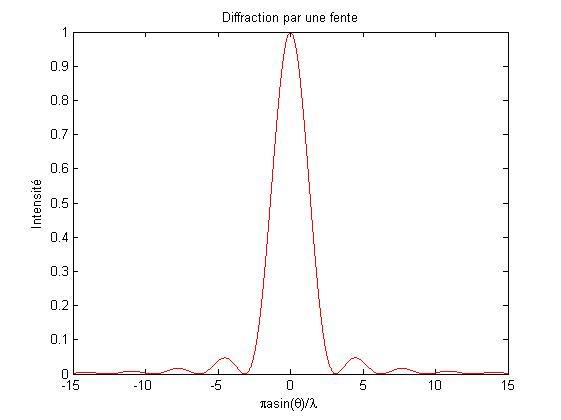
\includegraphics[scale=0.4]{diffraction1.jpg}
		\caption{Diffraction par une fente.}
		\label{fig:diffraction1}
	\end{subfigure}
	\begin{subfigure}[b]{0.45\textwidth}
		\centering
		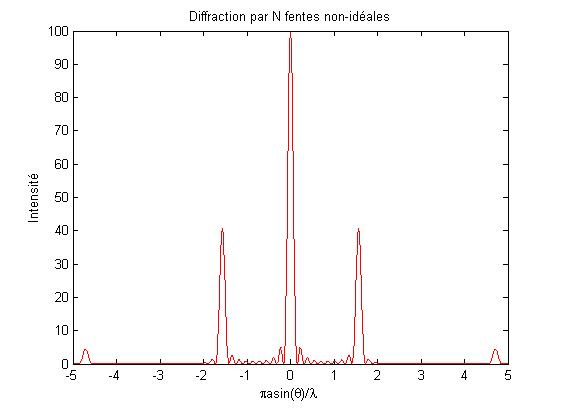
\includegraphics[scale=0.4]{diffraction3.jpg}
		\caption{Diffraction par $N$ fentes.}
		\label{fig:diffractionN}
	\end{subfigure}
	\caption{Intensité d'une onde diffractée par une fente et par $N$ fentes.}
\end{figure}

\subsubsection{Applications}
\paragraph{Mesure d'un objet de petite taille}
On peut effectuer la diffraction d'une onde par un objet de très petite
taille, par exemple un cheveu de largeur $a$. On va alors 
obtenir une figure d'intensité similaire à la figure \ref{fig:diffraction1}.
Sur cette figure, on peut mesurer les valeurs de $\theta$
où l'intensité s'annule et donc ensuite calculer $a$ via
\[ a\sin\theta = n\lambda.\]

\paragraph{Pouvoir séparateur (ou pouvoir de résolution spatiale)}
Le premier minimum de la figure d'intensité d'une
diffraction par une fente circulaire est donné
\[ D\sin\theta = 1.22\lambda\]
où $D$ est le diamètre de la fente et $\theta$ est
le pouvoir de résolution.

\section{Ondes stationnaire}
Une onde stationnaire est une onde pour laquelle ses nœuds ne bougent pas.
Elle est obtenue en fixant des nœuds ou des ventres à ses extrémités.
Son équation est la suivante
\[ \xi(x, t) = A \sin(kx) \cos(\omega t). \]

En général, un système supporte plusieurs modes\footnote{Dans un système
oscillatoire, un mode propre d'oscillation est une des fréquences auxquelles
un système excitable peut osciller après avoir été perturbé au voisinage
de son état d'équilibre stable.}, on a donc

$$\xi(x, t) = \sum_{m=1}^{\infty} A_m \sin(k_mx) \cos(\omega_m t).$$

%TODO modulation d'amplitude

\subsection{Battements}
La somme de deux ondes de fréquences différentes (mais proches)
$\omega_1$ et $\omega_2$ donne des battements (interférences se
déplaçant dans l'espace) La fréquence des battements
est donnée par

$$\frac{|\omega_1 - \omega_2|}{2}$$

Le principe de battements est illustré à la figure \ref{fig:battements}.
La somme des deux ondes (de \unit{30}{\hertz} et \unit{32}{\hertz})
est représentée en bleue, l'\emph{enveloppe} de leur somme est representée en rouge.
Sur la figure, on peut remarquer que la fréquence de l'enveloppe (qui est la
fréquence de battements), est bien $\frac{32-30}{2} = \unit{1}{\hertz}$.

\begin{figure}[ht!]
	\centering
	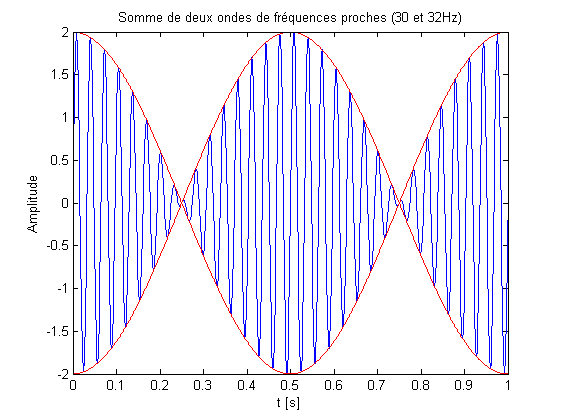
\includegraphics[scale=0.7]{battements.png}
	\caption{Illustration du principe de battements.}
	\label{fig:battements}
\end{figure}

\section{Émission}
L'émission d'une onde EM est obtenue en accélérant des charges.
Ce principe est utilisé dans les antennes élémentaires.

\subsection{Antennes}
Les antennes sont modélisées par des segments dans lequel un courant
alternatif circule (voir figure \ref{fig:antenne}.

% TODO : refaire avec circuitikz
\begin{figure}[ht]
	\centering
	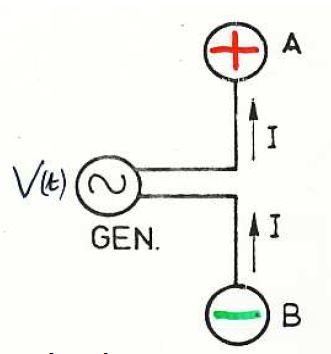
\includegraphics[scale=0.8]{antenne.jpg}
	\caption{Représentation schématique d'une antenne (expérience Hertz).}
	\label{fig:antenne}
\end{figure}

%Supposons que le segment soit aligné avec l'axe $z$.
%Il produit alors une onde électromagnétique partout dans le plan $xy$ mais
%dont l'amplitude est inversement proportionnelle à $R$ et l'intensité
%est inversement proportionnelles à $R^2$.
%
%Ce type d'antenne est une antenne dite demi longueur d'onde, elle émet
%donc une onde dont $\lambda = h/2$.
%
%Pour analyser l'interférence de plusieurs antennes,
%on fait l'approximation de Fraunhofer, voir section~\ref{sec:fraunhofer}.

\subsection{Délai/retard}
La vitesse de propagation d'une onde électromagnétique
$c$ n'est pas infinie. Il y a donc un temps de propagation
égal à $\frac{|\vec{r}|}{c}$ non-nul. Une onde arrivant
au point $P$ à l'instant $t$ dépend donc du rayonnement
de la source en $t' = t - \frac{|\vec{r}|}{c}$.

\subsection{Conservation d'énergie}
Autour d'une source ponctuelle de rayonnement électromagnétique
isotrope, la propagation est sphérique. Donc $E$ et $H$
sont proportionnels à $\frac{1}{r}$ et donc l'intensité rayonneée
est proportionnelle à $\frac{1}{r^2}$.
Or la loi de Coulomb prédit le rayonnement d'un
champ électrique proportionnel à $\frac{1}{r^2}$ autour
d'une charge ponctuelle. C'est parce que la loi
de Coulomb n'est valide que pour des particules
avec une accéleration nulle. Or dans une antenne les particules
ont une accéleration $\vec{a}$ non-nulle.

\subsection{Champ rayonné par une charge accélérée}
On peut observer les propriétés du champ $E$ rayonné suivantes :
\begin{itemize}
	\item Il est proportionnel à la charge $q$ ;
	\item Il est proportionnel à $\frac{1}{r}$ ;
	\item Il est nul dans la direction de $\vec{a}$ ;
	\item Il est non-nul dans les autres directions.
\end{itemize}
On peut donc écrire 
\[\vec{E}(t,\vec{r}) \propto \frac{q}{|\vec{r}|}\vec{a}_\perp(t')\]
où $\vec{a}_\perp = \vec{a}-(\vec{a}\cdot\vec{u}_r)\vec{u}_r$ et
$\vec{u}_r$ vecteur unitaire de direction $\vec{r}$\footnote{Autrement
dit, il s'agit de la composante perpendiculaire à $\vec{u}_r$ de $\vec{a}$.}. 
On peut également l'écrire de manière plus précise
\[\vec{E}(t,\vec{r}) = -\frac{\mu_0}{4\pi}\frac{q}{|\vec{r}|}\vec{a}_\perp(t-\frac{|\vec{r}|}{c}).\]
On retrouve ensuite facilement $\vec{H}(t,\vec{r})$ 
\[\vec{H}(t,\vec{r}) = \sqrt{\frac{\epsilon_0}{\mu_0}}\vec{u}_r \times \vec{E}(t,\vec{r}).\]

\subsection{Champ rayonné par un dipôle oscillant}
On considère ici un modèle simplifié dans lequel une charge
$-q$ est fixe tandis qu'une charge $+q$ oscille entre $-z_0$
et $z_0$ (voir figure \ref{fig:dipole}). Soit $P$ le point
d'intérêt. On définit $\vec{r'}$ le vecteur partant de $+q$ 
vers $P$ et $\vec{r}$ le vecteur partant de $-q$ vers $P$.
On a également un angle $\theta$, qui est l'angle entre l'axe
$OZ$ et $\vec{r}$ et un angle $\theta'$ (absent sur la figure)
qui est l'angle entre l'axe $OZ$ et $\vec{r'}$.

\begin{figure}[ht]
	\centering
	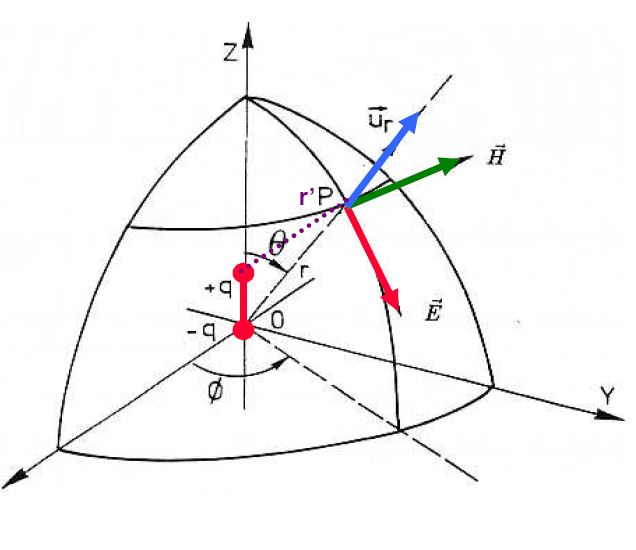
\includegraphics[scale=0.8]{dipole.jpg}
	\caption{Représentation schématique d'un dipôle oscillant.}
	\label{fig:dipole}
\end{figure}

La position de la charge $+q$ est donnée par 
\[z(t) = z_0\sin\omega t.\]
La moment dipolaire $p(t) \eqdef qz(t)$ est
donc donné par
\[p(t) = qz_0 \sin\omega t = p_0\sin\omega t.\]
Grâce à cela, on peut calculer l'accéleration
de la charge 
\[qa(t) = q\ffdif{z(t)}{t} = \ffdif{p(t)}{t} = -\omega^2p_0\sin\omega t.\]
Notons aussi que
\[\sin\omega t' = \sin\left(\omega(t-\frac{|\vec{r'}|}{c})\right) = \sin(\omega t - k|\vec{r'}|).\]
On prend ensuite deux hypothèses simplificatrices :
\begin{itemize}
	\item Le point $P$ d'observation du champ est très éloigné
	de la source, donc $\vec{r'} \approx \vec{r}$ et donc $\theta' = \theta$.
	On peut donc écrire $a_\perp = a\sin\theta$; 
	\item $z_0 << \lambda$ et donc $k\vec{r} \approx k\vec{r'}$. 
\end{itemize}
On a donc
\[\vec{E}(t,\vec{r'}) = -\frac{\mu_0}{4\pi}\frac{q}{|\vec{r'}|}\vec{a}_\perp(t')\]
que la première hypothèse nous permet de réecrire
\[\vec{E}(t,\vec{r}) = -\frac{\mu_0}{4\pi}\frac{q}{|\vec{r}|}\vec{a}(t')\sin\theta.\]
L'accélération calculée précédement et la seconde hypothèse nous permettent enfin de réecrire
\[\vec{E}(t,\vec{r}) = -\frac{\mu_0}{4\pi}\omega^2qz_0\frac{\sin\theta}{|\vec{r}|}\sin(\omega t -k|\vec{r}|)\vec{u}_\theta.\]
% FIXME : pas un souci de signe ici? J'aurais pas mis de "-" mais le formulaire en met un.
On retrouve ensuite très facilement
\[H_\phi = \sqrt{\frac{\epsilon_0}{\mu_0}}E_\theta\]
où $E_\theta$ est la norme de $\vec{E}(t,\vec{r})$.

\subsection{Champ rayonné par un élément de courant sinusoïdal}
On considère cette fois 2 charges $\pm q$ en mouvement
sinusoïdal opposé. On a donc
\[ p(t) = 2qz_0\sin(\omega t) = p_0\sin(\omega t).\]
Ce mouvement sinusoïdal de charge implique un courant
sinusoïdal $I(t)$.
% To be continued

%%%%%%%%%%%%%%%%%%%%%%%%%%%%
%	    QUANTIQUE          %
%%%%%%%%%%%%%%%%%%%%%%%%%%%%

\part{Physique quantique}
\section{Aspects corpusculaires des ondes électromagnétiques}
\subsection{Rayonnement du corps noir}
En physique, un corps noir désigne un objet idéal dont
le spectre électromagnétique ne dépend que la température.
Le corps noir aborbe toute l'enérgie électromagnétique
qu'il recevrait, sans en réfléchir ni en transmettre.
La lumière est donc totalement absorbée et le corps noir
apparaît... noir. Le corps noir peut cependant
émettre de la lumière s'il a une température
suffisamment élevée. Les observations expérimentales
montre que l'enérgie émise est proportionnelle à $\sigma T^4$
(Loi de Stefan-Boltzmann) et qu'il exisme un maxima $\lambda_m$
(traits discontinus bleus sur la figure \ref{fig:blackbody}).
La physique classique ne permet cependant pas d'expliquer
ces observations. En effet cette dernière prévoit une
énergie rayonnée $\propto \frac{1}{\lambda^4}$, et donc
une énergie infinie pour les faibles valeurs de $\lambda$
\footnote{Cette prédiction théorique est connue sous le nom
de ``catastrophe ultraviolette''.}.

\begin{figure}[ht]
	\centering
	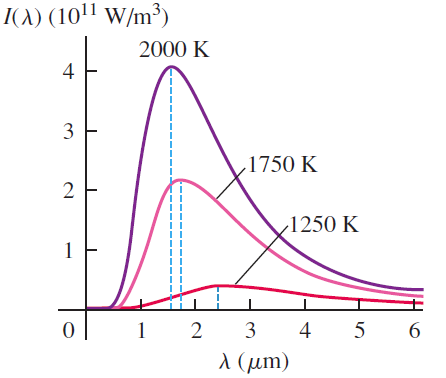
\includegraphics[scale=0.65]{blackbody.png}
	\caption{Graphe de l'émittance spectrale d'un corps
	noir en fonction de $\lambda$.}
	\label{fig:blackbody}
\end{figure}

Pour trouver une explication théorique valable, Planck
introduit l'idée de quantification de l'énergie :
l'énergie n'est pas émise de manière continue.
Un oscillateur de fréquence $f$ ne peut émettre
ou absorber de l'énergie que par paquets, par \textbf{quanta},
de valeur $E = hf$, où $h = \unit{6.626\cdot10^{-34}}{\meter\squared\kilo\gram\per\second}$.

\subsection{L'effet photo-électrique}
Une surface absorbant une lumière peut ``éjecter'' des électrons,
on appelle ça l'effet \emph{photo-électrique}.
Pour observer l'effet photo-électrique, considérons l'expérience
suivante. On place un système cathode/anode dans le vide. Ce système
est relié à un circuit électrique via lequel on peut mesurer le
photo-courant. La différence de potentiel entre l'anode et la
cathode est notée $V_{AC}$. En éclairant la cathode, celle-ci émet
des électrons avec différentes énergies cinétiques $\leq K_{\text{max}}$.
On peut chercher à annuler ce photo-courant en applicant un potentiel
d'arrêt $V_0 = -V_{AC}$ au système anode/cathode. En faisant de la sorte
on annule l'énergie cinétique des électrons, $K_{\text{max}} = eV_0$.
Comparons maintenant les prédictions du modèle ondulatoire de la lumière
avec les observations expérimentales.

\begin{tabular}{p{0.45\textwidth}|p{0.45\textwidth}}
	\textbf{Prédictions du modèle ondulatoire} & \textbf{Observations expérimentales} \\
	\hline
	L'intensité d'une onde EM ne dépend pas de sa fréquence. Le photo-courant
	ne devrait donc pas dépendre de la fréquence de la lumière.
	& Le photo-courant dépend de la fréquence de la lumière. Pour un
	matériau donné, on observe le photo-courant qu'à partir d'une
	certaine \textbf{fréquence seuil}. \\
	\hline
	Comme l'énergie reçue par la cathode dépend de l'intensité de la lumière,
	on s'attend à ce que le potentiel d'arrêt augmente avec l'intensité
	de la lumière. De plus, comme l'intensité ne dépend pas de la fréquence,
	on s'attend à ce que le potentiel d'arrêt n'en dépende pas non plus.
	& Le potentiel d'arrêt ne dépend pas de l'intensité mais bien de la
	fréquence. Plus la fréquence de la lumière est élevée, plus le potentiel
	d'arrêt augmente (cela signifie que l'énergie du photo-électron éjecté
	est plus grande). En augmentant l'intensité de la lumière, on augmente juste
	le nombre d'électrons par seconde et donc le photo-courant.
\end{tabular}

\paragraph{L'explication quantique}
Pour expliquer l'effet photo-électrique, Einstein
repris l'idée des quanta de Planck.
La lumière est composée de photons.
Chaque photon voyage à la vitesse de la lumière $c$.
Son énergie est appelée quanta et vaut
\[ E = hf = \frac{hc}{\lambda} .\]
Sa quantité de mouvement vaut
\[ p = mv = \frac{h}{\lambda} = \hbar k. \]

Ce postulat explique les observations expérimentales
faites précédemment :
\begin{enumerate}
	\item	Pour qu'un électron soit éjecté du matériau,
	l'énergie $hf$ apportée par le photon à
	l'électron doit être supérieure au travail d'extraction
	$\phi$ de l'électron dans ce matériau. On comprend donc
	l'existence d'une fréquence seuil $f = \frac{\phi}{h}$.
	\item Une plus grande intensité de la lumière signifie
	un plus grand nombre de photons par seconde absorbé,
	donc un plus grand nombre d'électrons par seconde éjecté,
	et donc un plus grand photo-courant.
	\item Enfin, on peut relier le potentiel d'arrêt à la
	fréquence en appliquant la conservation de l'énergie
	\[ K_{\text{max}} = eV_0 = hf - \phi .\]
\end{enumerate}

\subsection{La diffusion Compton}
Compton étudie la diffusion inélastique des rayons X
par la matière. On envoie de la lumière de longueur d'onde
$\lambda$ sur un électron au repos. On observe la longueur
d'onde $\lambda'$ de la lumière diffusée.

\begin{tabular}{p{0.45\textwidth}|p{0.45\textwidth}}
	\textbf{Prédictions du modèle ondulatoire} & \textbf{Observations expérimentales} \\
	\hline
	D'après la physique classique, la diffusion devrait être élastique, $\lambda = \lambda'$.
	& La lumière diffusée a une longueur d'onde différente, $\lambda' > \lambda$. On observe
	également que $\lambda'$ varie avec l'angle de de diffusion.
\end{tabular}

Le modèle des photons explique également ce caractère corpusculaire
de la lumière. En effet, en considérant les photons comme des
particules et en appliquant la conservation de la quantité
de mouvement, on trouve
\[ \lambda' -\lambda = \frac{h}{mc}(1-\cos\theta),\]
ce qui correspond à la formule trouvée expérimentalement.

\subsection{Le photon}
\subsubsection{Nature corpusculaire du photon}
\paragraph{Un photon est indivible}
Pour le démontrer, considérons
l'expérience illustrée à la figure \ref{fig:exp-photon1}.

\begin{figure}[ht!]
	\centering
	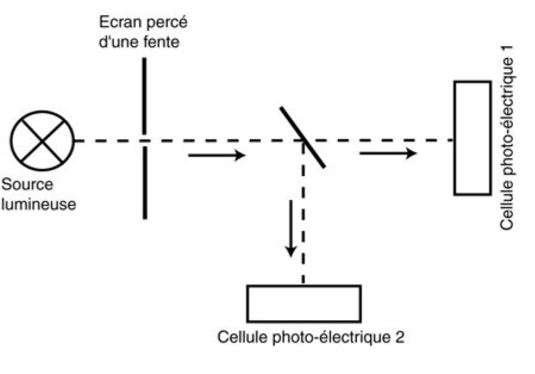
\includegraphics[scale=0.5]{exp_photon_1.jpg}
	\caption{Une source envoie de la lumière sur un miroir
	à travers une fente percée.}
	\label{fig:exp-photon1}
\end{figure}

En considérant les photons comme une onde, on peut prédire
que le faisceau se divisera en deux faisceaux d'intensité diminuée
de moitié et donc que l'énergie reçue à chaque cellule sera $\frac{1}{2}hf$.
En sachant que le seuil de sensibilité des cellules est $\approx hf$,
on ne devrait donc pas observer de courant. L'expérience
montre pourtant qu'un courant est créé sur les deux cellules mais
avec un nombre de photons par seconde diminué de moitié (par rapport
au cas ou tout le faisceau lumineux incident serait dirigé vers une seule
cellule). Ceci montre bien que le photon est indivisible.

\paragraph{Un photon conserve son énergie}
Pour le démontrer, considérons l'expérience illustrée
à la figure \ref{fig:exp-photon2}.

\begin{figure}[ht!]
	\centering
	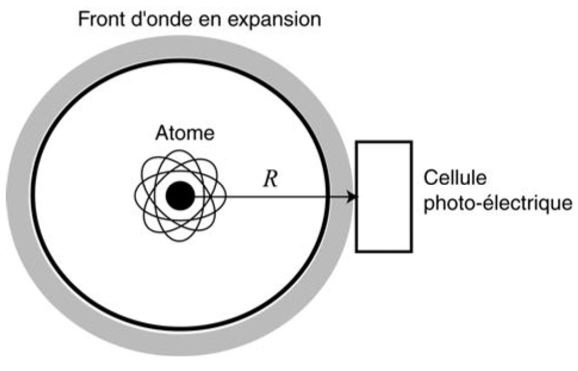
\includegraphics[scale=0.5]{exp_photon_2.jpg}
	\caption{Un atome (donc une source de rayonnement
	électromagnétique) situé à une distance $R$ d'une cellule
	photo-électrique.}
	\label{fig:exp-photon2}
\end{figure}

L'expérience consiste à mesurer le courant
sur la cellule photo-électrique en fonction de $R$.
En considérant le photon comme une onde électromagnétique,
on peut prédire que son énergie diminue en $\frac{1}{R^2}$. On s'attend
donc à ce qu'on ne puisse plus mesurer de courant sur
la cellule à partir d'une certaine distance.
L'expérience montre, même pour des distances énormes,
qu'un courant est toujours produit sur la cellule.
Le nombre de photons par seconde arrivant sur la cellule
diminue cependant en $\frac{1}{R^2}$.

\subsubsection{Nature ondulatoire du photon}
Bien qu'il se comporte parfois comme une particule,
le photon se comporte aussi comme une onde. On peut
en effet observer des phénomènes de diffraction de photons
et d'interférences entre photons.

\section{Aspects ondulatoires des particules}
\subsection{Ondes de ``de Broglie''}
Chaque particule est caractérisée par une masse au repos $m > 0$
et une vitesse $v$.

Une onde de Broglie lui est associée et vaut
\[ \lambda = \frac{h}{mv}. \]
Son énergie vaut
\[ E = hf = \hbar \omega. \]

\subsection{Diffraction des électrons}
Les électrons ayant un caractère ondulatoire, il
est possible d'étudier la diffractions des électrons
ou encore les interférences entre électrons. C'est l'objectif
de l'expérience des fentes de Young. L'expérience de
Young et le mystère quantique qui en découle sont
expliqués dans la vidéo ``Double Slit Experiment explained
by Jim Al-Khalili'' dont l'adresse est disponible dans
l'annexe \ref{sec:videos}.

Une des applications de la diffraction des électrons est
le microscope électronique, qui peut offrir une résolution
de \unit{0.1}{\nano\meter} à \unit{10}{\nano\meter}.
% TODO : expliquer le fonctionnement des microscopes électroniques

\subsection{Fonction d'onde}
Une particule est liée à une fonction d'onde.
L'amplitude de cette fonction d'onde, i.e. $|\Psi|^2$, peut être interprété
comme la \emph{densité} de probabilité par unité de volume de trouver
la particule à l'endroit de l'espace et au moment où cette fonction
d'onde est calculée.
C'est à dire que la probabilité de trouver une particule
au temps $t$ dans un parallélépipède rectangle de côtés
$\dif x$, $\dif y$ et $\dif z$ au point de coordonnée $(x, y, z)$ est
\[ |\Psi(x, y, z, t)|^2 \dif x \dif y \dif z .\]
Il est important de se rappeler que
\[ |z|^2 = z^{*} \cdot z \]
où $z^{*}$ est le conjugué de $z$.

On peut effectuer une séparation de variable sur la fonction d'onde,
\[ \Psi(\vec{r}, t) = \psi_1(\vec{r}) \cdot \psi_2(t). \]

\paragraph{Particule non-localisée}
Dans le cas d'une particule non-localisée, on a
\begin{align*}
\psi_1(\vec{r}) &= C_1(k)\exp(i\vec{k}\cdot\vec{r})
& \psi_2(t) &= C_2(E)\exp(-i\frac{E}{\hbar}t)
\end{align*}
où $C_1(k)$ et $C_2(E)$ sont des constantes.
Il y a plusieurs façons de voir que ces fonctions
correspondent à une particule non-localisée :
\begin{itemize}
	\item $\psi_1$ et $\psi_2$ sont des sinusoïdes
	pures. On peut donc définir, respectivement,
	leur nombre d'onde $k$ et leur fréquence $f$.
	La quantité de mouvement (resp. l'énergie) de
	la particule est donc bien définie
	et on a $\Delta p = 0$\footnote{En effet,
	comme $p = \hbar k$, $\Delta k = 0$ implique $\Delta p = 0$.}
	(resp. $\Delta E = 0$). Par le
	principe d'incertitude d'Heisenberg, on a alors
	$\Delta x = \infty$ (resp. $\Delta t = \infty$) ;
	\item $|\psi_1|^2 = C_1(k)$ et $|\psi_2|^2 = C_2(E)$. Ce
	qui signifie que la particule peut se trouver
	n'importe où dans l'espace (resp. dans le temps). ;
	\item $\psi_1$ et $\psi_2$ sont des sinusoïdes
	s'étendant de $-\infty$ à $+\infty$.
\end{itemize}
En pratique, on a toujours une idée de la
position d'une particule, elle se trouve dans
un espace connu.

\paragraph{Particule localisée}
Dans le cas d'une particule localisée, on a
\begin{align*}
\psi_1(\vec{r}) &= \int_{-\infty}^{+\infty} C_1(k)\exp(i\vec{k}\cdot\vec{r})
& \psi_2(t) &= \int_{-\infty}^{+\infty} C_2(E)\exp(-i\frac{E}{\hbar}t).
\end{align*}
Dans ces deux expressions, l'intégrale exprime ce qu'on
appelle une transformée de Fourier. C'est à dire que
$\psi_1$ et $\psi_2$ sont des sommes infinies de sinusoïdes
d'amplitude $C_1(k)$ et $C_2(E)$ de tout nombres d'onde et
de toute fréquences (et donc d'énergie).
En additionnant plusieurs sinusoïdes de nombres d'onde
différents (resp. de fréquences différentes),
on localise la fonction d'onde dans l'espace (resp.
dans le temps). Ce concept est illustré à la figure
\ref{fig:wave-packets} pour $\psi_1$.

\begin{figure}[ht!]
	\centering
	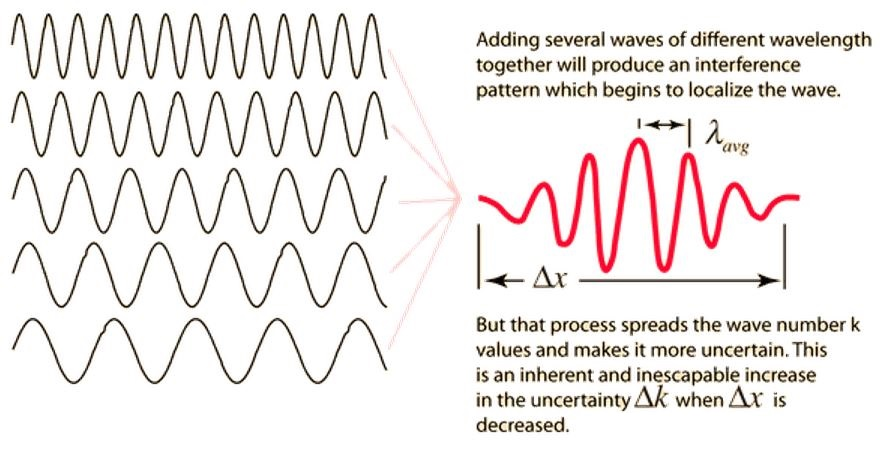
\includegraphics[scale=0.85]{wave_packets.jpg}
	\caption{Explication du concept de paquet d'ondes.}
	\label{fig:wave-packets}
\end{figure}

$C_1(k)$ peut être interprété comme la densité de probabilité
de présence d'une onde de nombre d'onde $k$. De même $C_2(E)$
peut être interpreté comme la densité de probabilité de
présence d'une onde d'énergie $E$. Ces distributions
peuvent être représentées par des fonctions gausiennes.
La largeur des ces fonctions gausiennes représente la
gamme de valeurs que peut prendre $k$ ou $E$. Plus la
gausienne sera large, plus l'imprécision sur $k$ (resp.
sur $E$) sera grande, plus la particule sera localisée
dans l'espace (resp. dans le temps).
Dans le cas d'une particule non-localisée, la largeur
de ces fonctions gausiennes est infinement petite. Ainsi,
$C_1(k)$ et $C_2(E)$ sont nulles partout sauf en un seul
point, ce qui signifie que $k$
et $E$ ne peuvent prendre qu'une seule valeur.
Les intégrales de la transformée de Fourier
redeviennent alors bien les expressions du paragraphe
précédent sur les particules non-localisées.

\section{Principe d'incertitude d'Heisenberg}
\begin{mynota}
  Posons l'opérateur $\Delta$ comme
  la grandeur de l’intervalle d'incertitude
  d'une grandeur physique.
\end{mynota}

On remarque que lorsqu'on a la fonction d'onde $\Psi$,
on a toutes les grandeur physiques intéressantes de la particule.
Mais on remarque aussi qu'une même particule,
en plus d'avoir une incertitude sur la position et le temps,
peut avoir une énergie $E$, une fréquence $f$,
une longueur d'onde $\lambda$, une vitesse $v$,
une quantité de mouvement $p$ et un nombre d'onde $k$ incertains.

\subsection{Le principe d'incertitude d'Heisenberg pour la position}
En effet, si tous les $C_1(k)$ sont non nuls,
$k$ peut valoir la valeur qu'il veut,
c'est à dire que
$\Delta k = \Delta p = \Delta v = \infty$.
Par contre, si $C_1(k)$ est non nul seulement
pour $k \in [-1;1]$, on a que
$\Delta k = 2$, $\Delta p = 2\hbar$ et $\Delta v = \frac{2\hbar}{m}$.

En fait, si $\Delta k = 0$, on remarque que
\[ |\psi_1(\vec{r})|
= \left|C_1(k) \exp\left(i\vec{r} \cdot \vec{k}\right)\right|
= \left|C_1(k)\right|\cdot\left|\exp\left(i\vec{r} \cdot \vec{k}\right)\right|
= C_1(k) \]
c'est à dire que la probabilité de trouver la particule est la même
quelle que soit la position.
On a donc $\Delta x = \infty$, $\Delta y = \infty$ et $\Delta z = \infty$.

De même, si on impose $\Delta x = 0$, il faut que $\psi_1(\vec{r})$ soit nul
partout sauf en un point (la position de la particule). Comme $\psi_1(\vec{r})$
est une transformée de Fourier, il faudra intégrer les sinus
sur un intervalle de longueur infinie pour obtenir
$\psi_1$ tel que $\psi_1(\vec{r})$ vaille 0 partout sauf en un seul point
donc $\Delta p_x = \infty$.

Le principe d'incertitude d'Heisenberg pour la position nous dit que
\begin{align*}
  \Delta x \cdot \Delta p_x \geq \frac{\hbar}{2}\\
  \Delta y \cdot \Delta p_y \geq \frac{\hbar}{2}\\
  \Delta z \cdot \Delta p_z \geq \frac{\hbar}{2}.
\end{align*}

Ce n'est donc pas un hasard qu'on ne puisse pas connaître en même temps
la position de la particule avec précision ainsi que sa quantité de mouvement.
Il est important de bien comprendre que cette inégalité n'est pas due
à des défauts des appareils de mesures mais est liée à la nature
ondulatoire des particules.

\subsection{Le principe d'incertitude d'Heisenberg pour le temps}
Le même raisonnement marche aussi pour $\psi_2$.
Si on connaît $f$, c'est à dire
que $\Delta E = \Delta f = 0$, on a
\[ |\psi_2(\vec{r})|
= \left|C_2(E) \exp\left(-i\frac{E}{\hbar}t\right)\right|
= \left|C_2(E)\right|\cdot\left|\exp\left(-i\frac{E}{\hbar}t\right)\right|
= C_2(E). \]
C'est à dire que la particule n'est pas localisée dans le temps, $\Delta t = \infty$.

Si on veut que la probabilité que la particule soit là qu'à un temps précis,
c'est à dire que $\Delta t = 0$,
comme $\psi_2$ est une transformée de Fourier, il faudra intégrer les sinus
sur un intervalle de longueur infinie
pour obtenir $\psi_2$ tel qu'il soit non nul que pour un certain $t$.
Donc, on aura $\Delta E = \infty$.

Le principe d'incertitude d'Heisenberg pour le temps nous dit que
\begin{align*}
  \Delta t \cdot \Delta E \geq \frac{\hbar}{2}.
\end{align*}

La plupart du temps, on travaille dans le cas où
$\Delta t = \infty$ et l'énergie est dans un état défini $\Delta E = 0$
(état stationaire)\footnote{C'est le
cas d'un électron autour d'un noyau d'atome par exemple.}.
On a alors
\[ \Psi(\vec{r}, t) = \psi_1(\vec{r}) \exp\left(-i\frac{E}{\hbar}t\right), \]

\section{L'équation de Schrödinger à une dimension}
Soit une particule de masse $m$ et d'énergie $E$ dans un potentiel $V(\vec{r})$,
on a l'équation suivante
\begin{align*}
	& \left[-\frac{\hbar^2\lap}{2m} + V(\vec{r},t)\right]\psi(\vec{r},t) = i\hbar\fpart{\psi(\vec{r},t)}{t}
	& \text{(dépendante du temps)}.
\end{align*}
La valeur de $|\psi(\vec{r},t)|^2$ varie donc en fonction du temps.
Comme expliqué précedemment, dans un grand nombre de cas, l'énergie
est dans un état défini, c'est à dire qu'on a
\[ \Psi(\vec{r},t) = \psi_1(\vec{r})\exp{-\frac{iEt}{\hbar}}.\]
Dans ce cas, on constate assez facilement que
\[ |\psi(\vec{r},t)|^2 = |\psi_1(\vec{r})|^2.\]
En substituant l'équation d'onde stationnaire dans
l'équation de Schrödinger dépendante du temps, on obtient l'équation
de Schrödinger indépendante du temps
\begin{align*}
	& \left[-\frac{\hbar^2\lap}{2m} + V(\vec{r})\right]\psi_1(\vec{r}) = i\hbar\fpart{\psi_1(\vec{r})}{t}
	& \text{(indépendante du temps)}.
\end{align*}

Une dérivation simple de ces équations est donnée en annexe \ref{sec:deriv-eq}

\paragraph{Paradoxe du chat de Schrödinger}
La vidéo ``What Is the Wave Function? - Instant Egghead \#50'' dont
l'adresse est donnée dans l'annexe \ref{sec:videos} explique
ce paradoxe.

% TODO : particule libre non-localisée/localisée
\subsection{Puits de potentiel 1D infini}
\label{sec:puits-1d}
On va résoudre l'équation de Schrödinger dans un puits infini,
c'est à dire avec
\[ U(x) = \left\{
  \begin{aligned}
    0 & \text{ si } x \in [0; L]\\
    \infty & \text{ sinon}.
  \end{aligned}
\right. \]
Dans l'intervalle $[0; L]$, $\psi_1(x)$ satisfait
l'équation
\[ -\frac{\hbar^2}{2m}\ffdif{\psi_1(x)}{x} = E\psi_1(x).\]
On a donc $\psi_1(x) = Ae^{ikx}+Be^{-ikx}$ où $A$ et $B$
sont définies par les conditons aux limites
\[ \left\{
  \begin{aligned}
    \psi_1(0) &=& 0 & \Rightarrow B = -A \Rightarrow \psi_1(x) = C\sin(kx)\\
    \psi_1(L) &=& 0 & \Rightarrow k = \frac{n\pi}{L}
  \end{aligned}
\right. \]
avec $n = 1, 2, \ldots$. En réinjectant $\psi_1(x) = C\sin(kx)$
dans l'équation de départ, on trouve $E = \frac{\hbar^2k^2}{2m}$
et donc
\begin{align*}
  E_n & = \frac{n^2h^2}{8mL^2} & n = 1, 2, \ldots.
\end{align*}
Cela signifie que le spectre d'énergie est \emph{discret}.
Il ne nous reste plus qu'à éliminer la constante $C$.
Pour cela, on va utiliser le fait que la particule doit
bien se trouver quelque part et donc imposer
\[ \int_{-\infty}^{\infty} |\psi_1(x)|^2 \dif x = 1.\]
Cette propriété de \emph{normalisation} permet de trouver
$C$. On trouve donc finalement
\begin{align*}
  {\psi_1}_n(x) & =
  \sqrt{\frac{2}{L}}\sin\left(\frac{n\pi x}{L}\right) & n = 1, 2, \ldots.
\end{align*}

\begin{myrem}
	On remarque que le niveau fondamental d'énergie (correspondant
	à $n=1$) n'est pas nul, contrairement à celui d'une particule
	classique dans le même potentiel. On peut comprendre cela en
	se servant du principe d'incertitude d'Heinsenberg. En effet,
	comme la particule est confinée, on a une certaine précision
	sur sa position : $\Delta x$ n'est donc pas infini. $\Delta p$
	ne peut donc pas être nul, et la particule a une certaine énergie.
	On comprend aussi pourquoi l'énergie augmente quand la longueur
	du puits diminue. De manière générale, tout confinement
	spatial d'une particule quantique conduit à la quantification
	de son spectre d'énergie.
	Comme la fonction d'onde est sinusoïdale, on remarque aussi
	que la probabilité de présence $|{\psi_1}_n(x)|^2$ peut valoir
	0 à certains endroits, ce qui est contraire à la physique
	classique.
\end{myrem}

\subsection{Puits de potentiel fini}
On résolvant l'équation de Schrödinger dans un puits
fini, c'est à dire avec
\[ U(x) = \left\{
  \begin{aligned}
    0 & \text{ si } x \in [0; L]\\
    U_0 & \text{ sinon}
  \end{aligned}
\right. \]
on remarque que $\psi_1(x)$ est non nul pour $x < 0$ et $x > L$
même s'il tend vers 0 tel une exponentielle, même si l'énergie de
la particule est inférieure à $U_0$. Ce phénomène,
appelée \emph{pénétration de barrière} est totalement
contraire à la physique classique!
L'énergie est à nouveau quantifiée et vaut
\[
  E_n = -\frac{\hbar^2\alpha_n^2}{2m}
\]
où $\alpha_n$ ne peut être déterminé que numériquement.

\begin{myrem}
	Cette situation correspond à un électron
	situé sur la surface d'un métal et qui a besoin
	d'une énergie $U_0$ pour s'en extraire.
\end{myrem}

\subsection{Puits de potentiel 3D infini}
On peut étendre la résolution de l'équation de Schrödinger
de la sous-section \ref{sec:puits-1d} à un cas 3D.
Soit une particule dans une boite de volume $V = L^3$,
avec
\[ U(x,y,z) = \left\{
  \begin{aligned}
    0 & \text{ si } x,y,z \in [0; L]\\
    \infty & \text{ sinon}.
  \end{aligned}
\right. \]
On trouve à nouveau que l'énergie est quantifiée
\begin{align*}
  E & = \frac{h^2(n_1^2+n_2^2+n_3^2)}{8mL^2} & n_1,n_2,n_3 = 1, 2, \ldots.
\end{align*}
La fonction d'onde générale est donnée par
\begin{align*}
  {\psi_1}_{(n_1,n_2,n_3)}(x) & =
  \sqrt{\frac{8}{L^3}}\sin\left(\frac{n_1\pi x}{L}\right)
											\sin\left(\frac{n_2\pi x}{L}\right)
											\sin\left(\frac{n_3\pi x}{L}\right)& n_1,n_2,n_3 = 1, 2, \ldots.
\end{align*}

On remarque qu'une particule peut avoir plusieurs états
quantiques distincts pour une même énergie. Par exemple,
les états $(n_1,n_2,n_3) = (2,1,1)$, $(1,2,1)$ et $(1,1,2)$
ont la même énergie mais des fonctions d'ondes différentes.
On appelle ça la \emph{dégénérescence}.
\subsection{Barrière de potentiel}
En résolvant l'équation de Schrödinger
aux alentour d'une barrière de potentiel,
c'est à dire avec
\[ U(x) = \left\{
  \begin{aligned}
    U_0 & \text{ si } x \in [0; L]\\
    0 & \text{ sinon}
  \end{aligned}
\right. \]
on remarque que même si $E < U_0$,
$\psi_1(x)$ est non-nul pour $x > 0$ et aussi pour $x > L$.
C'est à dire que la particule peut passer la barrière.
On appelle ça l'\emph{effet tunnel}.

En analysant le comportement de $\Psi$ en fonction du temps,
on remarque qu'il y a
une partie qui est réfléchie par la barrière de potentiel et
une partie qui passe à travers la barrière par l'effet tunnel.
Bien évidemment, plus $\frac{U_0}{E}$ est grand,
moins il y a de probabilité que l'électron passe à travers la barrière
et plus il y en a qu'il soit réfléchi.
A partir de la résolution de l'équation de Schrödinger, on
peut également calculer un coéfficient de transmission
\[ T = \frac{4E(U_0-E)}{4E(U_0-E)+U_0^2\sinh^2(\frac{L}{h}\sqrt{2m(U_0-E)})}.\]
Comme le montre la figure \ref{fig:tunnel}, l'effet
tunnel est vraiment contraire à la physique classique.

\begin{figure}[ht]
	\centering
	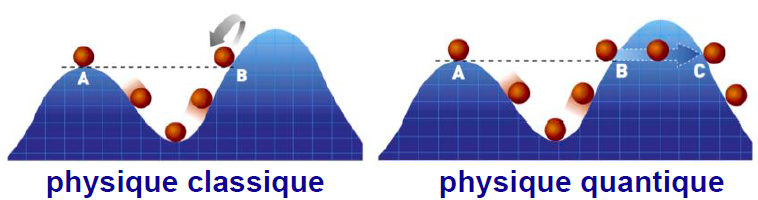
\includegraphics[scale=0.8]{tunnel.png}
	\caption{Comparaison de la physique classique et
	de la physique quantique par rapport à l'effet
	tunnel.}
	\label{fig:tunnel}
\end{figure}

\paragraph{Microscope à effet tunnel}
Une des applications de l'effet tunnel est le
microscope à effet tunnel. Son fonctionnement est expliqué dans
la vidéo ``Au-delà des nuages. Le microscope à effet tunnel''
dont l'adresse est donnée dans l'annexe \ref{sec:videos}.

\subsection{Oscillateur harmonique}
Le potentiel autour d'un atome en fonction de la distance
par rapport au noyau ressemble à une parabole (voir figure
\ref{fig:energy_level_osc}. C'est le potentiel d'un oscillateur
harmonique.

\begin{figure}[ht]
	\centering
	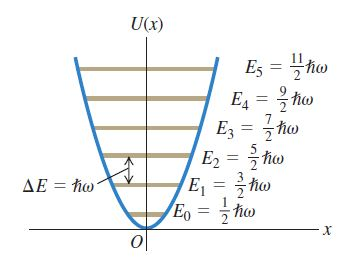
\includegraphics[scale=0.8]{energy_level_osc.jpg}
	\caption{Les niveaux d'énergie pour l'oscillateur
	harmonique.}
	\label{fig:energy_level_osc}
\end{figure}

En résolvant l'équation de Schrödinger avec ce potentiel,
on trouve que

\begin{align*}
  E_n & = \left(n+\frac{1}{2}\right)\hbar\omega & n = 0, 1, 2, \ldots.
\end{align*}

où $\omega = \sqrt\frac{k'}{m}$ et
$k'$ est la constante de raideur.

On peut remarquer que ces niveaux d'énergie sont équidistants et que
le niveau zéro est d'énergie non nulle. Les fonctions de probabilité 
de présence sont symétriques pour les niveaux impaires et antisymétriques 
pour les niveaux pairs. La figure \ref{fig:newton_vs_quantum_osc}
permet de comprendre une des différences principales entre
un oscillateur newtonien et un oscillateur quantique.

\begin{figure}[ht]
	\centering
	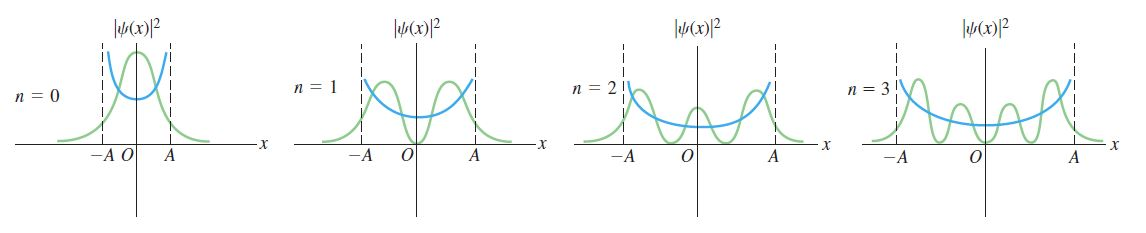
\includegraphics[scale=0.8]{newton_vs_quantum_osc.jpg}
	\caption{$A$ représente l'amplitude du mouvement de l'oscillateur
	newtonien avec le même niveau d'énergie. La ligne bleue représente
	la probabilité de présence pour l'oscillateur newtonien tandis que
	la ligne verte représente la probabilité de présence pour l'oscillateur
	quantique. On remarque pour l'oscillateur quantique, que la probabilité
	de présence au-delà de l'amplitude $A$ n'est pas nulle. A nouveau,
	c'est contraire à la physique classique !}
	\label{fig:newton_vs_quantum_osc}
\end{figure}

\section{Structure de l'atome}
% TODO : historique des modèles atomiques ?
\subsection{Structure atomique de l'hydrogène}
\subsubsection{Modèle de Bohr}
Le modèle de Bohr est complémentaire au modèle
planétaire de Rutherford qui décrit l'atome d'hydrogène
comme un noyau massif et chargé positivement, autour
duquel se déplace un électron chargé négativement.
Le problème de ce modèle est que l'électron, charge électrique
accélérée, devrait selon la physique classique rayonner
de l'énergie et donc finir par s'écraser sur le noyeau.
Niels Bohr propose alors d'ajouter :
\begin{enumerate}
	\item L'électron ne rayonne aucune énergie
	lorsqu'il se trouve sur une orbite stationnaire
	(cercles de diamètre quantifié - niveaux
	d’énergie précis). Ce sont les seules orbites
	sur lesquelles l'électron peut tourner à $v$ constant ;
	\item L'électron ne rayonne ou n’absorbe de
	l’énergie que lors d’un changement d’orbite.
\end{enumerate}
A partir de là, en écrivant les équations
de la conservation de l'énergie, de l'équilibre
des forces et de la conservation de la quantité de
mouvement et en émettant l'hypothèse\footnote{Suite aux
travaux de Planck.} que la quantité de mouvement est 
quantifié, Bohr parvient à quantifier l'énergie,
la rayon des orbites électroniques, et la vitesse
sur ces orbites.

\paragraph{Niveau d'énergie}
\[E_n = -\frac{1}{n^2}\frac{e^4m_{e-}}{2(4\pi\epsilon_0)^2\hbar^2}
= \frac{\unit{-13.6}{\electronvolt}}{n^2}\]
\paragraph{Rayon de la n-ième orbite électronique}
\[r_n = n^2\frac{4\pi\epsilon_0\hbar^2}{e^2m_{e-}} = n^2a_0\]
où $a_0 = \unit{5.297\cdot10^{-11}}{\meter} = 0.5397\dot{A}$.
Ce rayon est approximativement égal à la distance la plus
probable entre le proton et l'électron dans l'atome
d'hydrogène dans son état fondamental.
\paragraph{Vitesse de l'électron sur la n-ième orbite électronique}
\[v_n = \frac{e^2}{n\hbar 4\pi\epsilon_0} = \frac{1}{n}v_0\]
où $v_0 = \unit{2.214\cdot10^6}{\meter\per\second}$.
\paragraph{Validité du modèle de Bohr}
Le modèle de Bohr, bien qu'en accord avec l'expérience
du spectre discret d'émission et d'aborption de l'hydrogène (voir
figure \ref{fig:spectres-h}) n'est pas complet pour les raisons
suivantes :
\begin{itemize}
	\item Mélange de notions de physiques classiques et
	de physique quantiques ;
	\item Pas généralisable aux atomes qui possèdent
	plus d'un électron ;
	\item Ne permet pas d'expliquer les propriétés
	magnétiques de l'hydrogène ;
	\item Pas de notion de fonction d'onde et de densité
	de probabilité.
\end{itemize}

\begin{figure}[ht]
	\centering
	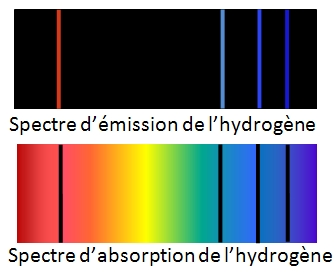
\includegraphics[scale=0.6]{spectres-h.jpg}
	\caption{En envoyant de la lumière blanche successivement
	sur de l'hydrogène gazeux, une fente et un prisme, on obtient
	des spectres d'émission et d'aborption discontinus. Cela signifie
	que l'énergie émise (resp. absorbée) par l'atome ne peut prendre
	que des valeurs discrètes, elle est quantifiée. Cette énergie
	permet à l'électron de s'éloigner (absorption du quantum)
	ou se rappocher du noyeau (émission d'un quantum).}
	\label{fig:spectres-h}
\end{figure}

\subsubsection{Nombres quantiques}
En résolvant l'équation de Schrödigner, on parvient à mettre en 
évidence 3 nombres quantiques :
\begin{align*}
	n 	&	\text{ nombre quantique principal} 	& n = 1,2,3,\dots \\
	l 	& \text{ nombre quantique orbital} 		& l = 0,1,2,\dots,,-1 \\
	m_l &	\text{ nombre quantique magnétique}	& m_l = 0,\pm 1,\pm 2,\dots,\pm l
\end{align*}

\paragraph{Spectre d'énergie}
Les niveaux d'énergie $E_n$ sont les mêmes que ceux
prédit par le modèle de Bohr. 
\paragraph{Moment angulaire}
La norme du moment angulaire $\vec{L}$ de l'électron est quantifiée
par le nombre quantique $l$
\[ |\vec{L}| = \sqrt{l(l+1)}\hbar. \]
La projection du moment angulaire sur un axe imposé $z$
est quantifiée par le nombre quantique $m_l$
\[ L_z = m_l\hbar. \]

\subsection{Orbitales atomiques}
En physique quantique, la notion d'orbitale atomique
est utilisée dans le modèle quantique de l'atome. 
Les électrons d'un atome ne sont plus en orbite circulaire
(contrairement au modèle de Bohr), mais occupent
de manière probabiliste certaines régions de l'espace
autour du noyau. On note les orbitales de
la manière suivante :

\begin{center}
  \begin{tabular}{c|ccccc}
    $l$ 		& 0 & 1 & 2 & 3 \\
    \hline
    Lettre 	& s & p & d & f \\
    Origine & {\bf s}harp & {\bf p}rincipal & {\bf d}iffuse & {\bf f}ondamental
  \end{tabular}
\end{center}

Les orbitales atomiques sont directement liées
à la probabilité de présence de trouver un électron
dans une ceraine zone d'espace autour du noyeau.

\paragraph{Probabilité de présence des électrons}
Pour trouver la probabilité de trouver un électron dans un atome
à une distance $r$ quand on connaît $\Psi(\vec{r})$,
il ne faut \emph{pas} faire $|\Psi(\vec{r})|^2 \dif r$
car comme on calcule maintenant $\Psi(\vec{r})$ en fonction des 3 dimension,
c'est la densité par volume.
Comme on est dans le cas d'une sphère, la formule de la probabilité
$P(r)$ de trouver l'électron à une distance entre $r$ et $r+\dif r$ est
\[ P(r) \dif r = |\Psi(\vec{r})|^2 \dif V
= |\Psi(\vec{r})|^2 4\pi r^2 \dif r. \]

\subsection{Spin de l'électron}
Le modèle avec 3 nombres quantiques est insuffisant
pour expliquer certaines observations expérimentales
\footnote{Effet Zeeman, séparation de certaines raies
spectrales.}. Pour explicuqer ces observations, il ne faut
plus considèrer l'électron comme une masse ponctuelle
mais bien comme une sphère en rotation : l'électron
a un moment angulaire de rotation intrinsèque, c'est
le \textbf{spin} de l'électron\footnote{La vidéo ``Petit
manège (Le spin des électrons)'' dont l'adresse est donnée
en annexe \ref{sec:videos} explique ce concept.}.
L'amplitude du moment angulaire de spin vaut
\[ |\vec{S}| = \sqrt{\frac{1}{2}(\frac{1}{2}+1)\hbar} 
= \sqrt{\frac{3}{4}}\hbar.\]
Sa composante $S_z$ est quantifiée par un nouveau
nomnbre quantique $m_s = \pm\frac{1}{2}$ (spin ``u''
ou ``down''), appelé le nombre quantique de spin
\[ S_z = m_s\hbar. \] 

\begin{myrem}
	Les particules de spin ``demi-entier'' comme les
	électrons, les protons et les neutrons sont des \textbf{fermions}.
	Les particules de spin ``entier'' comme les photons sont
	des \textbf{bosons}.
\end{myrem}

\subsection{Atomes à plusieurs électrons}
Un atome est composé d'un nombre $Z$ (nombre atomique)
d'électrons et de protons. Résoudre l'équation de Schrödinger
avec $Z$ électrons autour du noyeau est beaucoup plus complexe.
On fait donc l'approximation très grossièdre que l'électron
est seul autour d'un noyau de charge $Ze$.
L'énergie d'un électron est donc
\[ E_n \approx -\frac{Z_\mathrm{eff}^2}{(4\pi\perm_0)^2}\frac{m_ee^4}{2n^2\hbar^2}
= -Z_\mathrm{eff}^2\frac{\si{13.6}{\electronvolt}}{n^2} \]
où $m_e$ est la masse d'un électron, $e$ sa charge et
$Z_\mathrm{eff}$ la charge qu'il subit réellement,
c'est-à-dire sa charge effective.
Plus précisément, 
\[ Z_\mathrm{eff} = Z - S \] 
où $S$ est le nombre d'électrons des couches inférieures (les électrons de non-valence).
Les électrons d'une même couche principale subissent donc tous la même charge effective.

Par exemple, pour un atome de $15$ protons dont la configuration 
électronique est $1s^2 2s^2 2p^6 3s^2 3p^3$, le 12\ieme{} électron
appartient à la troisième couche ($n=3$), $S$ vaut donc $10$ et 
$Z_\mathrm{eff} = 15 - 10 = 5$.

\subsection{Principe d'exclusion de Pauli}
Deux électrons ne peuvent pas avoir les mêmes 4 nombres quantiques
$n$, $l$, $m_l$ et $m_s$. Cela implique une limitation du nombre
d'électrons par couche. La couche $n=1$ accepte 2 électrons,
la couche $n=2$ accepte 8 électrons et la n-ième couche
accepte $2n^2$ électrons.
Ce principe n'est donc utile que dans le cas de plusieurs électrons.

% TODO : tableau périodique des élements

\section{Molécules et matière condensée}
\subsection{Liaisons chimiques}
On distingue deux grandes catégories de
liaison chimique :
\begin{enumerate}
	\item Liaisons forte, $\unit{1}{\electronvolt} \leq E_{\text{liaison}} \leq \unit{5}{\electronvolt}$ :
	\begin{itemize}
		\item Liaison ionique : interaction entre ions de charge opposée ;
		\item Liaison covalente : mise en commun d'un nombre égal d'électrons ;
		\item Liaison métallique (cristaux).
	\end{itemize}
	\item Liaisons faibles, $E_{\text{liaison}} < \unit{1}{\electronvolt}$
	\begin{itemize}
		\item Liaison de Van der Waals : interaction entre dipôle électrique ;
		\item Liaison ``hydrogène'' : interaction en atome d'hydrogène polarisée
		positivement et un autre atome (O, N, F) polarisée négativement.
	\end{itemize}
\end{enumerate}

\paragraph{Pourquoi les atomes se lient?}
Selon la physique classique, les atomes se lient
pour atteindre un niveau d'énergie plus bas.
La section suivante étudie de manière quantique
les liaisons chimiques.

\subsection{Modèle du cation hydrogène}
Le cation hydrogène est le système ``moléculaire''
le plus simple : 2 protons et 1 électron (voir figure 
\ref{fig:cation-h2}).

\begin{figure}[ht]
	\centering
	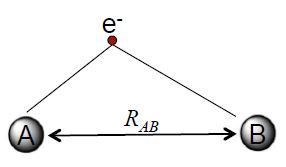
\includegraphics{cation_h2.jpg}
	\caption{Système moléculaire le plus simple : 2 protons
	et 1 électron.}
	\label{fig:cation-h2}
\end{figure}

Il faut donc résoudre l'équation de Schrödinger
moléculaire pour ce système. La fonction d'onde (orbitale moléculaire)
est une combinaision linéaire d'orbitales atomiques
\[ \psi = a\psi_A + b\psi_B. \]
En élevant au carré cette fonction d'onde pour
obtenir la probabilité de présence de l'électron, on
fait apparaitre 3 termes :
\begin{itemize}
	\item $a^2\psi_A^2$ : probabilité de trouver l'électron
	près de $A$ ;
	\item $b^2\psi_B^2$ : probabilité de trouver l'électron
	près de $B$ ;
	\item $2ab\psi_A\psi_B$ : probabilité de trouver l'électron
	entre $A$ et $B$ : \textbf{liaison}.
\end{itemize}
Comme il n'y a pas de raison que l'électron soit plus près
de $A$ que de $B$ et inversement, on impose $a^2\psi_A^2=b^2\psi_B^2$
et on obtient $a = \pm b$. On a donc finalement
deux solutions pour l'équation de Schrödinger :
\begin{itemize}
	\item $\psi = a(\psi_A+\psi_B)$ : orbitale moléculaire \textbf{liante}
	(figure \ref{fig:liante}) ;
	\begin{figure}[ht]
		\centering
		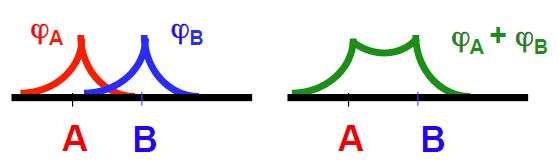
\includegraphics[scale=0.8]{orb-liante.jpg}
		\caption{Orbitale moléculaire liante.}
		\label{fig:liante}
	\end{figure}
	\item $\psi = a(\psi_A-\psi_B)$ : orbitale moléculaire
	\textbf{anti-liante} (figure \ref{fig:anti-liante}).
	\begin{figure}[ht]
		\centering
		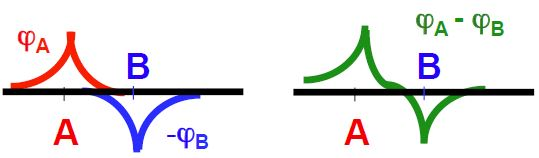
\includegraphics[scale=0.8]{orb-anti-liante.jpg}
		\caption{Orbitale moléculaire anti-liante.}
		\label{fig:anti-liante}
	\end{figure}
\end{itemize}
En normalisant la probabilité de présence on trouve $a = \frac{1}{\sqrt{2}}$.

D'un point de vue énergétique, on peut dire qu'en se
recouvrant, les deux orbitales atomiques de même énergie
donnent naissance à deux orbitales moléculaires d'énergies
différentes, l'une liante stabilisée et l'autre anti-liante
déstabilisée.

\subsection{Orbitales moléculaires}
Pour remplir les orbitales moléculaire on applique
simplement le principe d'exclusion de Pauli et
la règle de Hund, c'est à dire qu'un électron
est placé dans chaque orbitale moléculaire de
même énergie avant d'apparier deux électrons sur
un même niveau énergétique.

\subsection{Spectroscopie moléculaire}
La spectroscopie moléculaire étudie l'absorption
et l'émission d'une onde électro-magnétique par 
des molécules. Tout comme les transition entre niveaux
d'énergie dans les atomes entrainent un spectre atomique,
les transitions entre niveaux d'énergie de vibration
et de rotation des molécules entrainent un spectre moléculaire. 
Chaque molécule a donc une \textbf{signature}.
Dans cette sous-section, nous nous concentrons sur les
molécules diatomiques.

\paragraph{Energie de rotation}
Un premier modèle de molécule diatomique est repris
sur la figure \ref{fig:mol-dia1}. On peut calculer
son énergie de rotation
\[ E_l = l(l+1) \frac{\hbar}{2m_rr_0^2} \]
où $r_0$ est la distance entre les deux atomes.

\begin{figure}[ht]
	\centering
	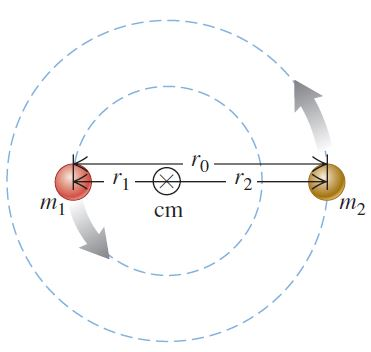
\includegraphics[scale=0.7]{mol-dia1.jpg}
	\caption{Une molécule diatomique est modélisée
	comme deux masses ponctuelles $m_1$ et $m_2$
	séparées par une distance $r_0$. La distance entre
	ces masses et le centre de masse de la molécules
	sont $r_1$ et $r_2$.}
	\label{fig:mol-dia1}
\end{figure}

\paragraph{Energie de vibration}
Dans le modèle précédent, on considère que la molécule est
rigide, ce n'est pas vraiment le cas. On prend donc un autre modèle
représenté à la figure \ref{fig:mol-dia1} et on calcule
son énergie de vibration
\[ E_n = \left(n + \frac{1}{2}\right)\hbar\sqrt\frac{k'}{m_r} \]
où $k'$ est la constante de raideur de la vibration et
$m_r$ est la masse réduite des masses des deux atomes $m_1$ et $m_2$ valant
\[ m_r = \frac{m_1m_2}{m_1+m_2}. \]

\begin{figure}[ht]
	\centering
	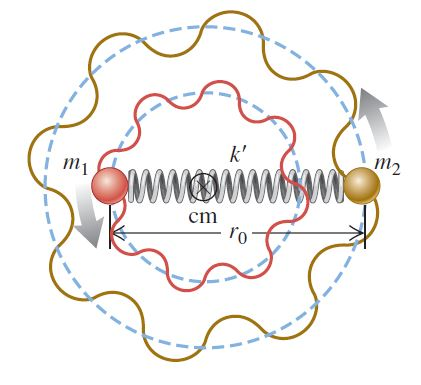
\includegraphics[scale=0.7]{mol-dia2.jpg}
	\caption{Modèle d'une molécule diatomique non-rigide.}
	\label{fig:mol-dia2}
\end{figure}

\paragraph{Spectre complet}
\[ E_{n,l} = l(l+1)\frac{\hbar^2}{2m_rr_0^2} + (n+\frac{1}{2})\hbar\sqrt{\frac{k'}{m_r}} \]
Les transitions entre niveaux d'énergie doivent suivrent certaines
règle de sélection :
\begin{align*}
	\Delta n = \pm 1 & \text{ et } & \Delta l = \pm 1.
\end{align*}

\subsection{Physique du solide}
Dans la matière condensée (solide ou liquide)
les distances inter-atomiques sont comprises entre
\unit{0.5}{\nano\meter} et \unit{0.1}{\nano\meter}.
Les interactions inter-atomiques sont fortes.
Les atomes d'un solide s'arrangent en réseau cristalin,
c'est à dire une répétition périodique d'une structure
cristallographique dans tout l'espace.
On distingue plusieurs types de solides selon
le type des liaison :
\begin{itemize}
	\item Les solides ioniques : liaisons ioniques $\pm$
	directionnelles ;
	\item Les solides covalents : liaisons covalentes
	directionnelles ;
	\item Les solides métalliques : liaisons homogènes
	et isotropes et électrons délocalisés.
\end{itemize}

% TODO : potentiel périodique

\subsection{Théorie des bandes}
Dans un solides,
les électrons sont mis en communs entre les différents atomes.
On remarque que les électrons ne peuvent avoir leur énergie que dans certains
intervalles qu'on appelle bande.
Le principe d'exclusion de Pauli s'applique ici aussi et donc certaines
bandes peuvent être remplies et ne plus accepter d'électrons.
La dernière bande remplie est appelée la bande de valence et la suivante
bande de conduction.
La longueur de la bande interdite entre les deux est appelée
band gap et est notée $E_g$.

S'il n'y a pas exactement le bon nombre d'électron pour
que la bande de valence soit remplie et que la bande de conduction soit
vide, il y en a dans la bande de conduction.
La séparation entre les bandes pleines et vides, et égale à $E_F$,
l'énergie de Fermi.
Les électrons présents dans une bande partiellement remplie sont libres de se
déplacer facilement dans cette bande. Le courant peut donc passer facilement.
On dit que le solide est un \emph{conducteur}.

Sinon, si $E_g$ est élevé, de l'ordre de 2 à \si{6}{\electronvolt},
on dit que c'est un \emph{isolant}.
Si $E_g$ est plus faible, on dit que c'est un \emph{semi-conducteur}.

\begin{figure}[ht]
	\centering
	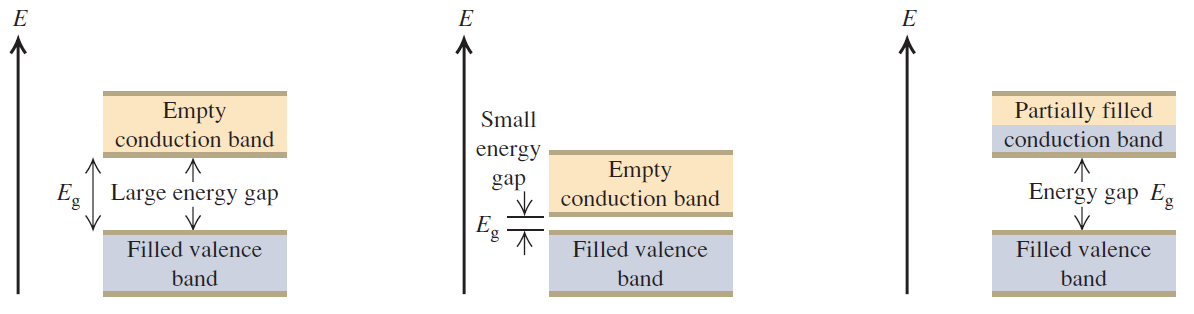
\includegraphics[scale=0.8]{band.png}
	\caption{Illustration du concept de bandes d'énergies.
	A gauche, un isolant. Au centre, un semi-conducteur. A droite
	un conducteur.}
\end{figure}

La théorie des bandes est expliquée dans la vidéo 
``L'électron libre. La théorie des bandes''
dont l'adresse est donnée en annexe \ref{sec:videos}.
\subsection{Semi-conducteur}
Pour les semi-conducteurs,
si la température passe au dessus de \si{0}{\kelvin},
il y a une probabilité que les électrons
se trouvent sur la bande de conduction,
un petit courant peut donc passer.

La distribution des électrons est donnée par la distribution de Fermi-Dirac
(voir figure \ref{fig:fermi-dirac} :
\[ f(E) = \frac{1}{1+\exp\left(\frac{E-E_F}{k_BT}\right)}. \]
où $E_F$ est l'énergie de Fermi et est défini telle que
$f(E_F) = \frac{1}{2}$.

\begin{figure}[ht]
	\centering
	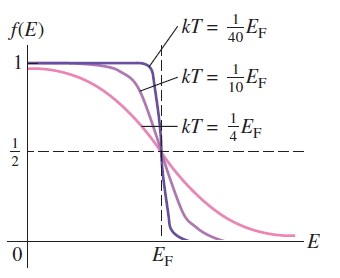
\includegraphics[scale=0.8]{fermi-dirac.png}
	\caption{Graphe de la distribution de Fermi-Dirac.}
	\label{fig:fermi-dirac}
\end{figure}

\subsubsection{Conduction intrinsèque dans les semi-conducteurs}
Lorsqu'un électron est excité, il peut passer de la bande de valence
à la bande de conduction, laissant derrière lui un \emph{trou}.
Sous l'effet d'un champ électrique un électron d'un atome voisin 
peut alors venir combler ce trou, laissant un autre trou derrière lui. 
Les électrons et les trous (que l'on peut assimiler à des charges positives)
se déplacent, il y a donc un courant intrisèque dans les semi-conducteurs.
Dans les semi-conducteurs pures, le nombre de trou dans la bande de valence
$N_{h+}$ est égal au nombre d'électrons dans la bande de conduction $N_{e-}$.
% TODO : add figure
\subsubsection{Dopage}
Le dopage des semi-conducteurs consiste en l'ajout d'impuretés.
Prenons l'exemple ici d'un semi-conducteur composé de Germanium,
un atome tétravalent.

\paragraph{Dopage N}
Le dopage N consiste à ajouter des atomes pentavalents
(par exemple l'Arsenic) de sorte que $N_{e-} >> N_{h+}$, 
la conduction est donc faite via les électrons et on appelle
cela un semi-conducteur de type N (N pour négatif).
% TODO : add figure
\paragraph{Dopage P}
Le dopage P consiste à ajoutet des atomes trivalents
(par exemple le Gallium) de sorte que $N_{e-} << N_{h+}$,
la conduction est donc faite vie les trous et on appelle
cela un semi-conducteur de type P (P pour positif).
% TODO : add figure
% TODO : P-N junction diode and field effect transistor

\appendix
\section{Rappels d'analyse vectoriel}
Définissons avant tout l'opérateur $\nabla$
\[ \nabla  \eqdef (\fpart{}{x}, \fpart{}{y}, \fpart{}{z}).\]
\subsection{Divergence}
\paragraph{Définition} 
La divergence de $\vec{F}$ égale le flux sortant de $\vec{F}$ 
au travers d'une boîte infinitésimale par unité de volume
\[ {\rm div}{\vec{F}} = \lim_{\Delta V \to 0} \frac{\oint{\vec{F}\cdot\dif\vec{S}}}{\Delta V}.\]
Autrement dit : si la divergence est non nulle en un point, alors le flux est
non nul autour de ce point et celui-ci absorbe ou est une source de champ.
\paragraph{Notation}
\[ {\rm div}{\vec{F}} = \nabla\cdot\vec{F} = \fpart{F_x}{x} + \fpart{F_y}{y} + \fpart{F_z}{z}\]

\subsection{Rotationnel}
\paragraph{Définition}
Le rotationnel de $\vec{F}$ égale la circulation d'un vecteur
par unité de surface
\[ \vec{{\rm rot}}{\vec{F}} = \lim_{\Delta S \to 0} \frac{\oint{\vec{F}\cdot\dif\vec{l}}}{\Delta S}.\] 
\paragraph{Notation}
\[ \vec{{\rm rot}}{\vec{F}} = \nabla\times\vec{F} = (\fpart{F_z}{y}-\fpart{F_y}{z})\hat{i}
+ (\fpart{F_x}{z}-\fpart{F_z}{x})\hat{j} + (\fpart{F_y}{x}-\fpart{F_x}{y})\hat{k}\]

\section{Unités}
En physique quantique, il y a deux unités souvent utilisées:
\begin{itemize}
\item le Hartree ($1Ha =  4,36\cdot 10^{-18} J$)
\item le \AA ngstr\"om ($1 \AA = 10^{-10} m$)
\end{itemize}

\section{Dérivation simple des équations de Schrödinger}
\label{sec:deriv-eq}
\paragraph{Indépendante du temps}
Premièrement, on calcule l'énergie de la particule
\[ E = E_{\text{cin}} + E_{\text{pot}} = \frac{mv^2}{2} + U = \frac{p^2}{2m} + U.\]
On considère ensuite une fonction d'onde quelconque $\psi = e^{i(kx-\omega t)}$
que l'on va dériver deux fois par rapport à $x$ :
\[ \fpart{\psi}{x} = ik\psi ,\]
\[ \ffpart{\psi}{x} = (ik)^2\psi. \]
Or, on a $p = \frac{h}{\lambda} = \hbar k$ et donc $k = \frac{p}{\hbar}$.
En substituant dans $\ffpart{\psi(x)}{x}$, on obtient
\[ \ffpart{\psi}{x} = -\frac{p^2}{\hbar^2} \Rightarrow p^2 =
-\frac{\hbar^2}{\psi}\ffpart{\psi}{x}.\]
Enfin, en substituant cette valeur de $p^2$ dans l'équation de l'énergie
multiplié par $\psi$, on obtient bien
\[ -\frac{\hbar^2}{2m}\ffdif{\psi}{x} + U(x)\psi = E\psi.\]

\paragraph{Dépendante du temps}
Premièrement, on calcule l'énergie $E = \hbar\omega = hf$ et on
considère une fonction d'onde quelconque $\psi = e^{i(kx-\omega t)}$
que l'on va dériver par rapport à $t$ :
\[ \fpart{\psi}{t} = -i\omega\psi \Rightarrow \omega = \fpart{\psi}{t}\frac{i}{\psi}.\]
En isolant $\omega$ dans l'équation de l'énergie, on obtient $\omega = \frac{E}{\hbar}$
que l'on peut égaler à l'autre valeur de $\omega$ trouvant en dérivant $\psi$ :
\[ E\psi = i\hbar\fpart{\psi}{t}.\]
Or, on a déjà trouvé une équation pour $E\psi$ lors de la dérivation de l'équation
de Schrödinger indépendante du temps, on obtient donc finalement
\[ i\hbar\fpart{\psi}{t} = -\frac{\hbar^2}{2m}\ffdif{\psi}{x} + U(x)\psi.\]

\section{Vidéos des CM de physique quantique}
\label{sec:videos}
\begin{itemize}
	\item Double Slit Experiment explained by Jim Al-Khalili :
	\url{http://youtu.be/A9tKncAdlHQ} ;
	\item Le yin et le yang (La dualité onde-particule) :
	\url{http://youtu.be/N968DgSVLkg} ;
	\item L'électron dans tous ses états :
	\url{http://youtu.be/9Uf_LNULgeo} ;
	\item Au-delà des nuages. Le microscope à effet tunnel :
	\url{http://youtu.be/HaqNSbQA0hs} ;
	\item Le microscope à effet tunnel :
	\url{http://youtu.be/NEsbREz-BBU} ;
	\item What Is the Wave Function? - Instant Egghead \#50
	(Schrödinger's cat) : \url{http://youtu.be/aowYf44gDRY} ;
	\item Petit manège (Le spin des électrons) :
	\url{http://youtu.be/tcpBwgN5hlE} ;
	\item L'électron libre. La théorie des bandes :
	\url{http://youtu.be/EWLgeBVY-08}.
\end{itemize}
\end{document}
